% Section 5 transcription. Source wording and mathematical errors retained.
% See section_5_errors.txt for the separate review.
\setcounter{section}{4}
\section{Complex Numbers}

\begin{ILOssec}
\item \ILOf
\end{ILOssec}

% Main deck slide 2

\subsection{Introduction to complex numbers}
\label{sec:complex_intro}

\begin{learningoutcomes}
\item Define real, imaginary and complex numbers and the complex conjugate
\item Plot complex numbers on an Argand diagram
\end{learningoutcomes}

% Main deck slide 3

Consider the equation ${z}^{2}-8z+15=0$. Completing the square
\begin{align*}
    {\left(z-4\right)}^{2}-1 &=0 \\
    z-4 &= \pm 1 \\
    \therefore z &=4\pm 1
\end{align*}
and so $z=3$ or $z=5$. 

Now, consider the equation ${z}^{2}-8z+17=0$. Completing the square again
\begin{align*}
{\left(z-4\right)}^{2}+1 &=0 \\
z-4 &= \pm \sqrt{-1} \\
\therefore z &=4\pm \sqrt{-1} \; .
\end{align*}
The solution does not exist, \textit{i.e.} it has no ‘real’ roots. These two quadratics are plotted in figure \ref{fig:quadratics}.
\begin{figure}
    \centering
    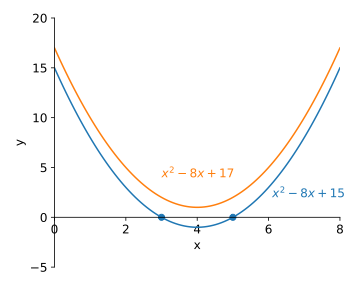
\includegraphics[width=0.5\linewidth]{Figures/Section5/quadratic_roots.png}
    \caption{The blue line shows the example quadratic with two real roots, indicated by the dots. The orange line shows the example case with no real roots. }
    \label{fig:quadratics}
\end{figure}

Let's imagine that $\sqrt{-1}$ does exist, by which we mean that it is some quantity that we can manipulate algebraically. We define
\begin{align}
    i=\sqrt{-1} \; .
\end{align}
Here $i$ is an ``imaginary'' number. You might also see this called $j$ (but not in this course). Any multiple of $i$ is also an imaginary number \textit{e.g.} $3i$, $\sqrt{2}i$, $\frac{4i}{5}$, $\pi i$ are all imaginary numbers. 

\goodbreak
\begin{example}[DIY]
\label{ex:511}
Express the solution to the following equations in terms of $i$
\[
{z}^{2}=-1 \qquad \qquad {w}^{2}=-16 \qquad \qquad {v}^{2}=-28
\]
\end{example}

\begin{blanksol}
\begin{align*}
    z=\pm \sqrt{-1} &=\pm i \\
    w=\pm \sqrt{16}\sqrt{-1} &=\pm 4i \\
    v=\pm \sqrt{28}\sqrt{-1} &=\pm 2\sqrt{7}i
\end{align*}
\end{blanksol}

Return to the equation ${z}^{2}-8z+17=0$. We arrived at $z=4\pm \sqrt{-1}$ or $ z=4\pm i$. This is a \textbf{complex number}. In \textbf{standard form}, a complex number is written as
\begin{align}
    z=x+yi \; .
\end{align}
It has a real part and an imaginary part $\operatorname{Re}\left(z\right)=x$ and $\operatorname{Im}\left(z\right)=y$. \textbf{Note:} The imaginary part is a real number!

\textbf{The Argand diagram} Figure \ref{fig:complex_number_lines} shows how a complex number can be understood as a two-dimensional number, consisting of a real part, which is on the real number line, and an imaginary part, which is on the imaginary number line.
\begin{figure}
    \centering
    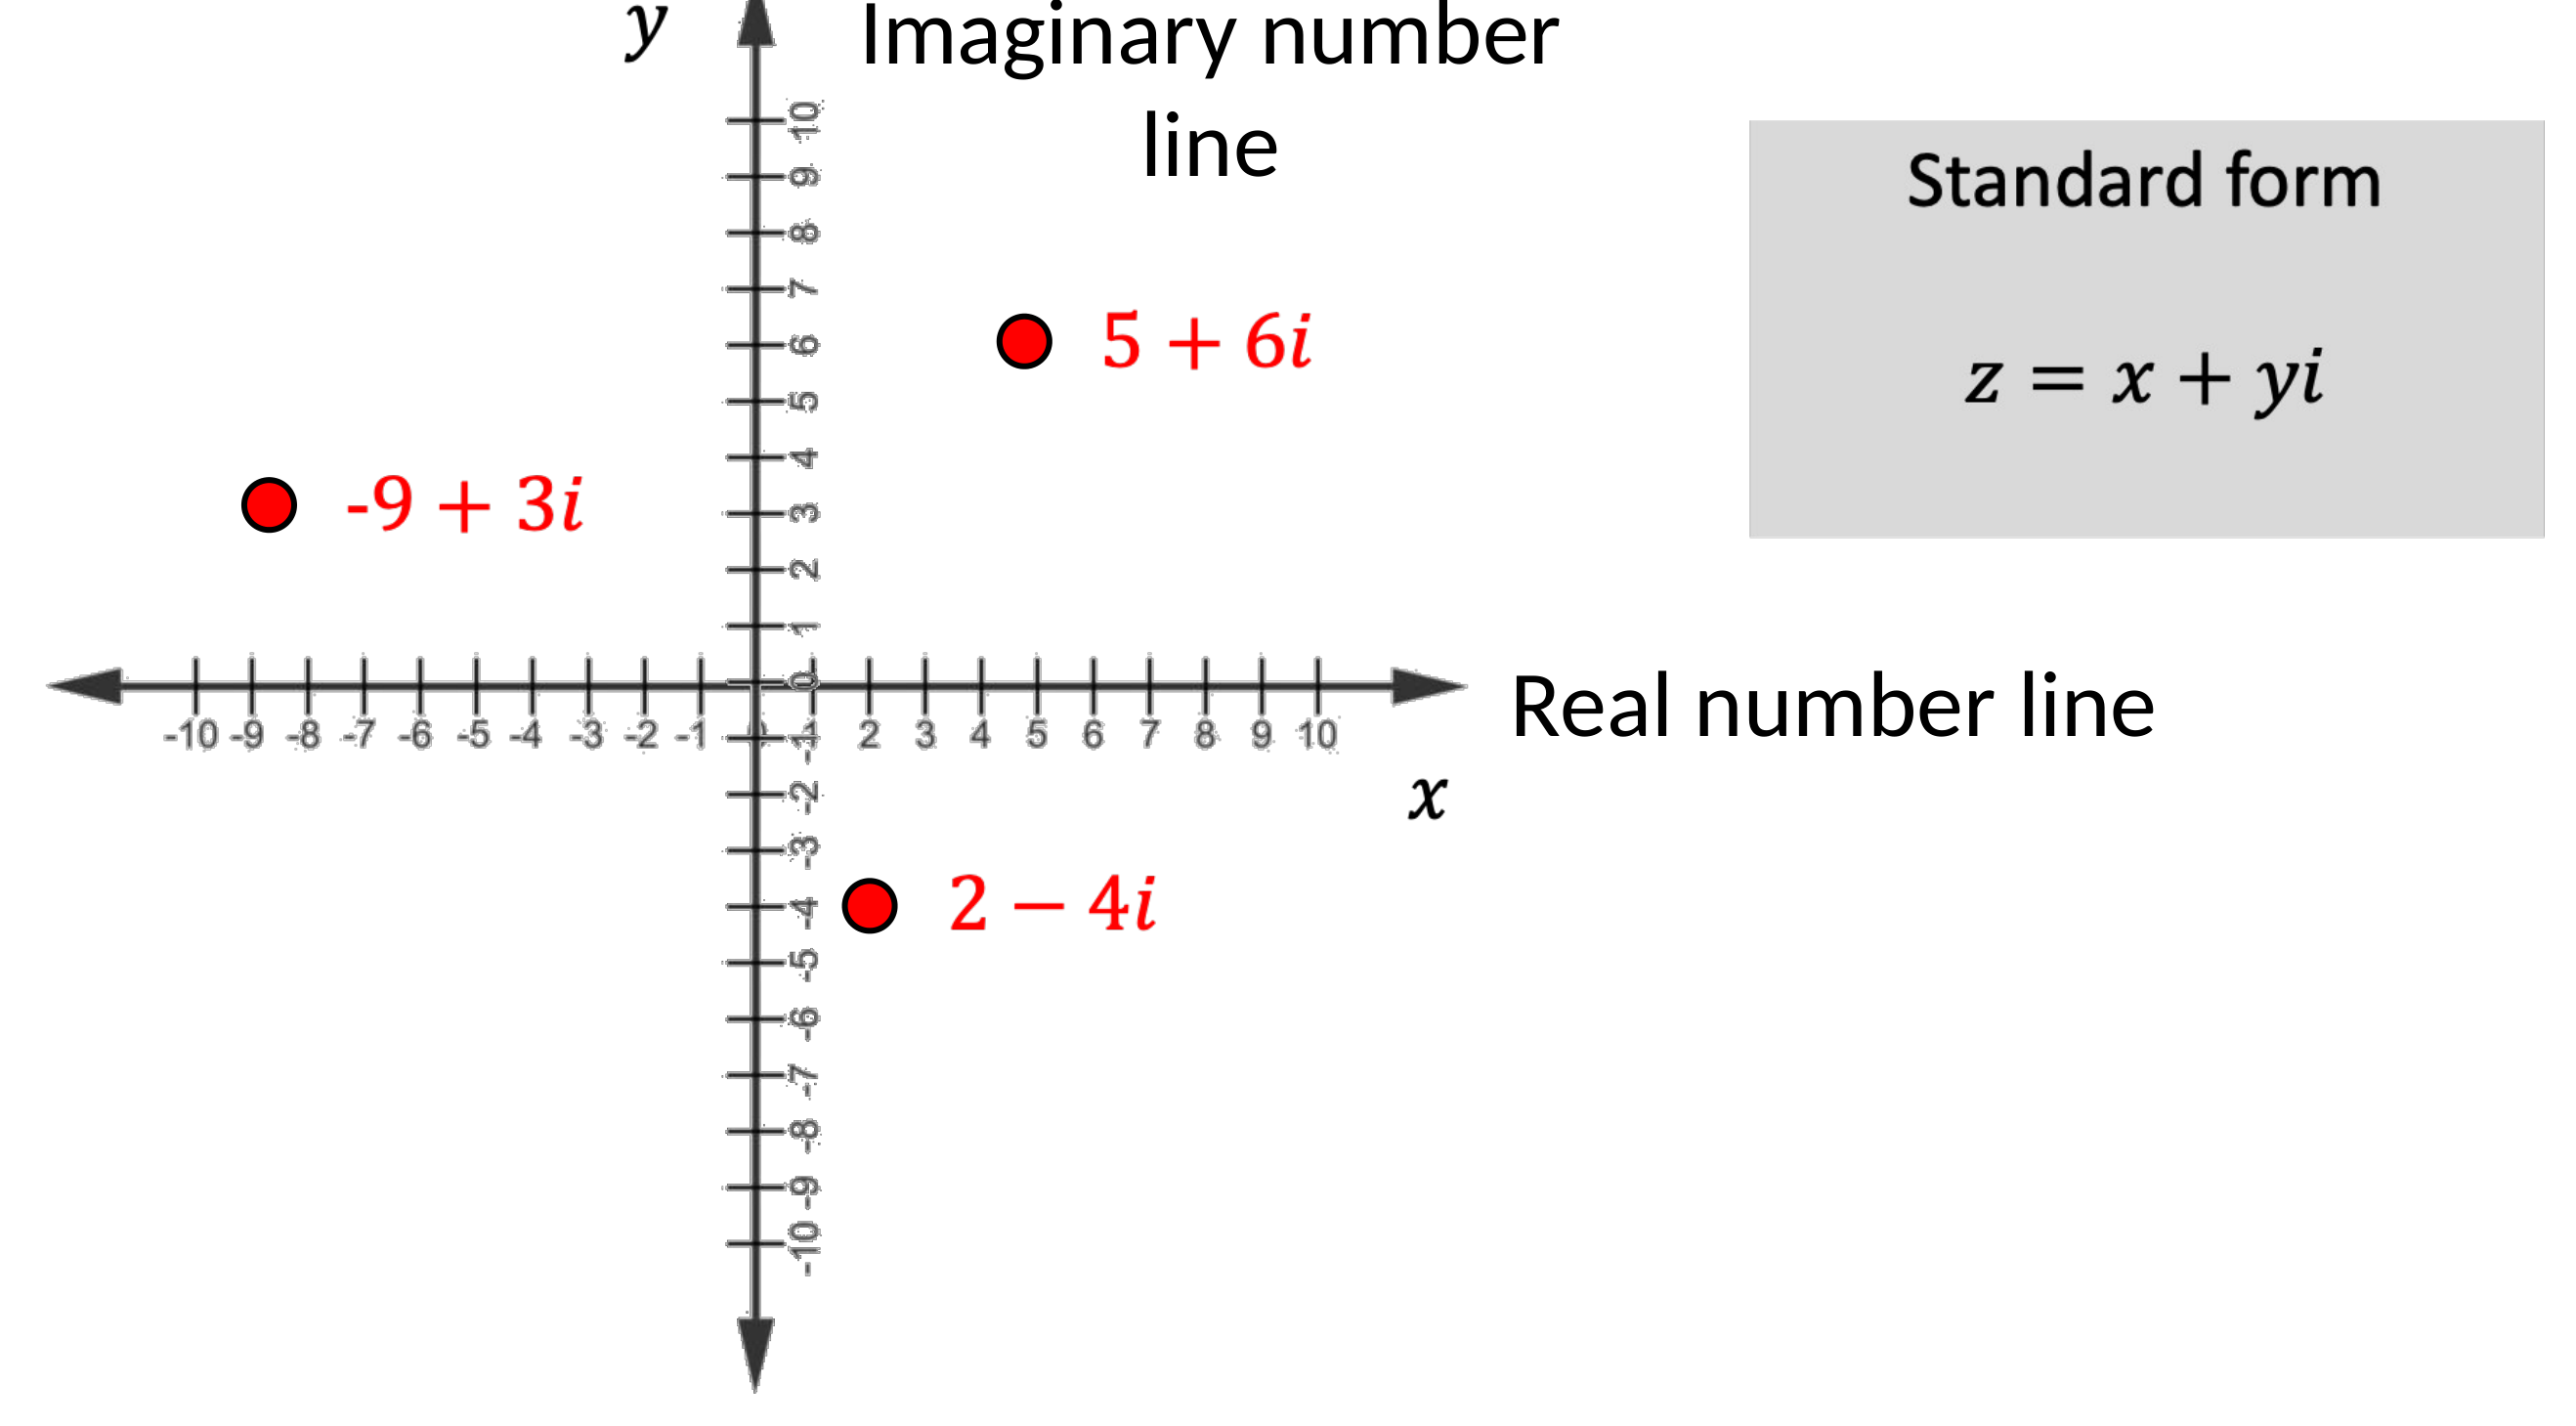
\includegraphics[width=0.75\linewidth]{Figures/Section5/complex_number_lines.png}
    \caption{Complex numbers are comprised of two numbers ($x$ and $y$ in standard form), each of which can take any value on the number line. }
    \label{fig:complex_number_lines}
\end{figure}

Figure \ref{fig:argand_diagram}(a) shows an \textbf{Argand Diagram}. It plots the real part of a complex number on the horizontal axis and the imaginary part on the vertical axis.

% Main deck slide 11
\textbf{The complex conjugate} Every complex number $z=x+yi$ has its (complex) \textbf{conjugate} $\overline{z}=x-yi$. To find the conjugate, reverse the sign of the imaginary part. The conjugate is used in some operations e.g. division of complex numbers. It is also sometimes denoted ${z}^{\ast }$.

\goodbreak
\begin{example}[Lecture]
\label{ex:512}
For the following complex numbers, find
\begin{enumerate}[label=(\alph*)]
\item their real and imaginary parts
\item their complex conjugates
\end{enumerate}
\[
{z}_{1}=2+5i \qquad \qquad {z}_{2}=-7-2i
\]
Then plot ${z}_{1},{z}_{2},{\overline{z}}_{1},{\overline{z}}_{2}$ on an Argand Diagram.
\end{example}

\begin{solution}
    The real parts are $\operatorname{Re}\left({z}_{1}\right)=\blank{2}$ and $\operatorname{Re}\left({z}_{2}\right)=\blank{-7}$. The imaginary parts are $\operatorname{Im}\left({z}_{1}\right)=\blank{5}$ and $\operatorname{Im}\left({z}_{2}\right)=\blank{-2}$. The conjugates are ${\overline{z}}_{1}=\blank{2-5i}$ and ${\overline{z}}_{2}=\blank{-7+2i}$.
    \ifcsname insertBlanks\endcsname
        \begin{center}
        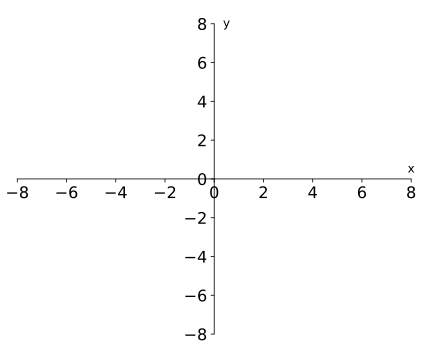
\includegraphics[width=.6\linewidth]{Figures/Section5/example_512_axes.png}
        \end{center}
    \else
        \begin{center}
        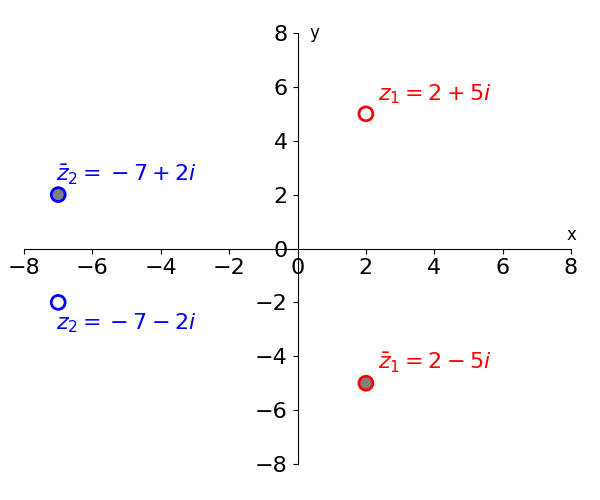
\includegraphics[width=.6\linewidth]{Figures/Section5/example_512.png}
        \end{center}
    \fi
\end{solution}
% Main deck slide 14

\goodbreak
\begin{recap}{\ref{sec:complex_intro}}
\item $i=\sqrt{-1}$ is an imaginary number (as is any multiple of $i$)
\item A complex number is the sum of a real and imaginary number and can be written in standard form as $z=x+yi$
\item An Argand Diagram plots the real part of a complex number on the x-axis and the imaginary part on the y-axis
\item Taking the conjugate of a complex number means reversing the sign of the imaginary part, i.e. $\overline{z}=x-yi$
\end{recap}

% Main deck slide 15

\newtexpage
\subsection{Arithmetic of complex numbers}
\label{sec:complex_arithmetic}

\begin{learningoutcomes}
\item Add, subtract, multiply, and divide complex numbers in standard form.
\item Find the magnitude of a complex number.
\end{learningoutcomes}

% Main deck slide 16

\textbf{Addition and subtraction of complex numbers.} For complex number arithmetic, we can treat $i$ like a variable. Consider two complex numbers
\begin{align*}
    {z}_{1} &= {x}_{1}+{y}_{1}i \\
    {z}_{2} &= {x}_{2}+{y}_{2}i \; .
\end{align*}
These can be added together by adding the real parts and the imaginary parts separately
\begin{align*}
{z}_{1}+{z}_{2} &=\left({x}_{1}+{y}_{1}i\right)+({x}_{2}+{y}_{2}i) \\
&= {\left({x}_{1}+{x}_{2}\right)} + {\left({y}_{1}+{y}_{2}\right)}i
\end{align*}

The same is true for subtraction, subtract the real parts and imaginary parts separately
\[
{z}_{1}-{z}_{2}={\left({x}_{1}-{x}_{2}\right)} + {\left({y}_{1}-{y}_{2}\right)}i \; .
\]

\textbf{Multiplication and division of complex numbers.} Consider two complex numbers ${z}_{1}={x}_{1}+{y}_{1}i$ and ${z}_{2}={x}_{2}+{y}_{2}i$. These can be multiplied by expansion
\begin{align*}
{z}_{1}{z}_{2} &=\left({x}_{1}+{y}_{1}i\right)\left({x}_{2}+{y}_{2}i\right) \\
&={x}_{1}{x}_{2}+\left({x}_{1}{y}_{2}+{x}_{2}{y}_{1}\right)i+{y}_{1}{y}_{2}{i}^{2} \\
&={\left({x}_{1}{x}_{2}-{y}_{1}{y}_{2}\right)} + {\left({x}_{1}{y}_{2}+{x}_{2}{y}_{1}\right)} i \; ,
\end{align*}
where in going from the second to the third line we used the definition $i^2 = -1$.

\begin{figure}
    \centering
    \subfig{0.44}{Figures/Section5/argand_diagram.png}{${\rm Re}(z)$ and ${\rm Im}(z)$.}
    \subfig{0.52}{Figures/Section5/complex_modulus.png}{$|z|$.}
    \caption{Two plots of a complex number on an Argand diagram. (a) The real part is the $x$-coordinate and the imaginary part is the $y$-coordinate. (b) The modulus is the distance from the origin.}
    \label{fig:argand_diagram}
\end{figure}

The \textbf{modulus} or \textbf{magnitude} of a complex number is $\left|z\right|=\sqrt{z\overline{z}}$ Defining $z=x+yi$
\begin{align}
\begin{split}
    \left|z\right| &=\sqrt{(x+yi)(x-yi)} \\[4pt]
    &=\sqrt{{x}^{2}+{y}^{2}} \; .
\end{split}
\end{align}
Therefore, $|z|$ is the distance from the origin on the Argand diagram, as shown in figure \ref{fig:argand_diagram}(b).

Consider again the two complex numbers ${z}_{1}={x}_{1}+{y}_{1}i$ and ${z}_{2}={x}_{2}+{y}_{2}i$, the quotient is also a complex number
\[
\frac{{z}_{1}}{{z}_{2}}=\frac{{x}_{1}+{y}_{1}i}{{x}_{2}+{y}_{2}i} \, , 
\]
however it is not immediately clear how to write it in standard form. Compare this to dividing ${z}_{1}$ by a real number $a$
\[
\frac{{z}_{1}}{a}=\frac{{x}_{1}+{y}_{1}i}{a}=\frac{{x}_{1}}{a}+\frac{{y}_{1}}{a}i \; .
\]
In this case it is straightforward to write this in standard form. 

In the case of $z_1/z_2$, we can always turn the complex number in the denominator $z_2$ into a real number by multiplying top and bottom by $\overline{{z}_{2}}$

\begin{align}
\frac{{z}_{1}}{{z}_{2}}&=\frac{{z}_{1}\overline{{z}_{2}}}{{z}_{2}\overline{{z}_{2}}} = \frac{{z}_{1}\overline{{z}_{2}}}{{\left|{z}_{2}\right|}^{2}} \; .
\end{align}
We can now use the rules of complex number multiplication to write this quotient in standard form
\[
\frac{{z}_{1}}{{z}_{2}}=\frac{({x}_{1}+{y}_{1}i)({x}_{2}-{y}_{2}i)}{{\left({x}_{2}\right)}^{2}+{\left({y}_{2}\right)}^{2}} = {\frac{{x}_{1}{x}_{2}+{y}_{1}{y}_{2}}{{\left({x}_{2}\right)}^{2}+{\left({y}_{2}\right)}^{2}}} + {\frac{{x}_{2}{y}_{1}-{x}_{1}{y}_{2}}{{\left({x}_{2}\right)}^{2}+{\left({y}_{2}\right)}^{2}}}i \; .
\]

\goodbreak
\begin{example}[Lecture]
\label{ex:521}
Given the two complex numbers ${z}_{1}=-3+4i$ ${z}_{2}=5-5i$ find

(a) ${z}_{1}+{z}_{2}$ and ${z}_{1}-{z}_{2}$ \qquad (b) ${z}_{1}{z}_{2}$ \qquad (c) $\frac{{z}_{1}}{{z}_{2}}$
\end{example}
\begin{solution}
\begin{align*}
\text{(a)}\quad {z}_{1}+{z}_{2} = \blank{\left(-3+5\right)+\left(4-5\right)i}&=\blank{2-i}\\
{z}_{1}-{z}_{2} = \blank{\left(-3-5\right)+\left(4+5\right)i} &=\blank{-8+9i}
\end{align*}
\begin{align*}
\text{(b)}\quad {z}_{1}{z}_{2} &=\blank{\left(-3+4i\right)\left(5-5i\right)}\\
&=\blank{-15+20i+15i-20{i}^{2}} =\blank{5+35i} \; .
\end{align*}
\begin{align*}
\text{(c)}\quad \frac{{z}_{1}}{{z}_{2}} &=\frac{\left(-3+4i\right)}{\left(5-5i\right)} = \blank{\frac{\left(-3+4i\right)(5+5i)}{\left(5-5i\right)(5+5i)}} \\
&=\blank{\frac{\left(-15+20i-15i+20{i}^{2}\right)}{50}} =\blank{\frac{-35+5i}{50}=-\frac{7}{10}+\frac{1}{10}i}
\end{align*}
\end{solution}

% Main deck slide 24
\goodbreak
\begin{example}[Video]
\label{ex:522}
Find the complex values of $z$ that satisfy the equation
\[
z\overline{z}+11z+9\overline{z}+3-8i=0
\]
\end{example}

\begin{solution}
First write $z=x+yi$, such that $\overline{z}=\blank{x-yi}$ and sub. in
\begin{align*}
    \blank{\left(x+yi\right)\left(x-yi\right)+20x+2yi+3-8i}&=0 \\[4pt]
    \therefore \blank{{x}^{2}+{y}^{2}+20x+3+\left(2y-8\right)i}&=0
\end{align*}
Taking the imaginary part of both sides gives $\blank{2y-8=0}$ so $y=\blank{4}$.

Taking the real part of both sides gives $\blank{{x}^{2}+{y}^{2}+20x+3=0}$ or $\blank{{x}^{2}+20x+19} =0$, which factorises to
\[
\blank{\left(x+19\right)\left(x+1\right)}=0
\]
and so $x=\blank{-19}$ or $x=\blank{-1}$. Putting it all together this means $z=-\blank{1+4i}$ or $z=\blank{-19+4i}$
\end{solution}

% Main deck slide 25
\goodbreak
\begin{recap}{\ref{sec:complex_arithmetic}}

\item The imaginary number $i$ can be treated like a variable where ${i}^{2}=-1$

\item To add complex numbers, simply add their real and imaginary parts.

\item To multiply, expand out and collect the real and imaginary parts.

\item To divide, multiply both numerator and denominator by the conjugate of the denominator, so that the denominator becomes a real number.

\item The magnitude of a complex number $z=x+yi$ is $\left|z\right|=\sqrt{{x}^{2}+{y}^{2}}$.

\end{recap}

% Main deck slide 26

\newtexpage
\subsection{Polar and Exponential Forms}
\label{sec:complex_polar}

\begin{learningoutcomes}
\item Convert complex numbers between standard, polar, and exponential forms
\item Perform multiplication, division and power operations with complex numbers in polar and exponential form
\end{learningoutcomes}

% Main deck slide 27

Consider a point (a complex number) on an Argand diagram. We can convert this point to polar coordinates (see figure \ref{fig:polar} using the relations
$x=r \cos \theta$, $y=r \sin \theta $, $r=\sqrt{{x}^{2}+{y}^{2}}$, and $\tan \theta =\frac{y}{x}$. Thus, the complex number $z = x + yi $ can be written in polar form as
\begin{align}
    z = x+yi = r(\cos \theta +i\sin \theta ) \; ,
\end{align}
where $r=\left|z\right|$ is the modulus or magnitude of the complex number $\theta =\operatorname{Arg}(z)$ (normally $-\pi \leq \theta \leq \pi $ or $0 \leq \theta \leq 2\pi$ ) is the argument of the complex number.

\begin{figure}[h]
    \centering
    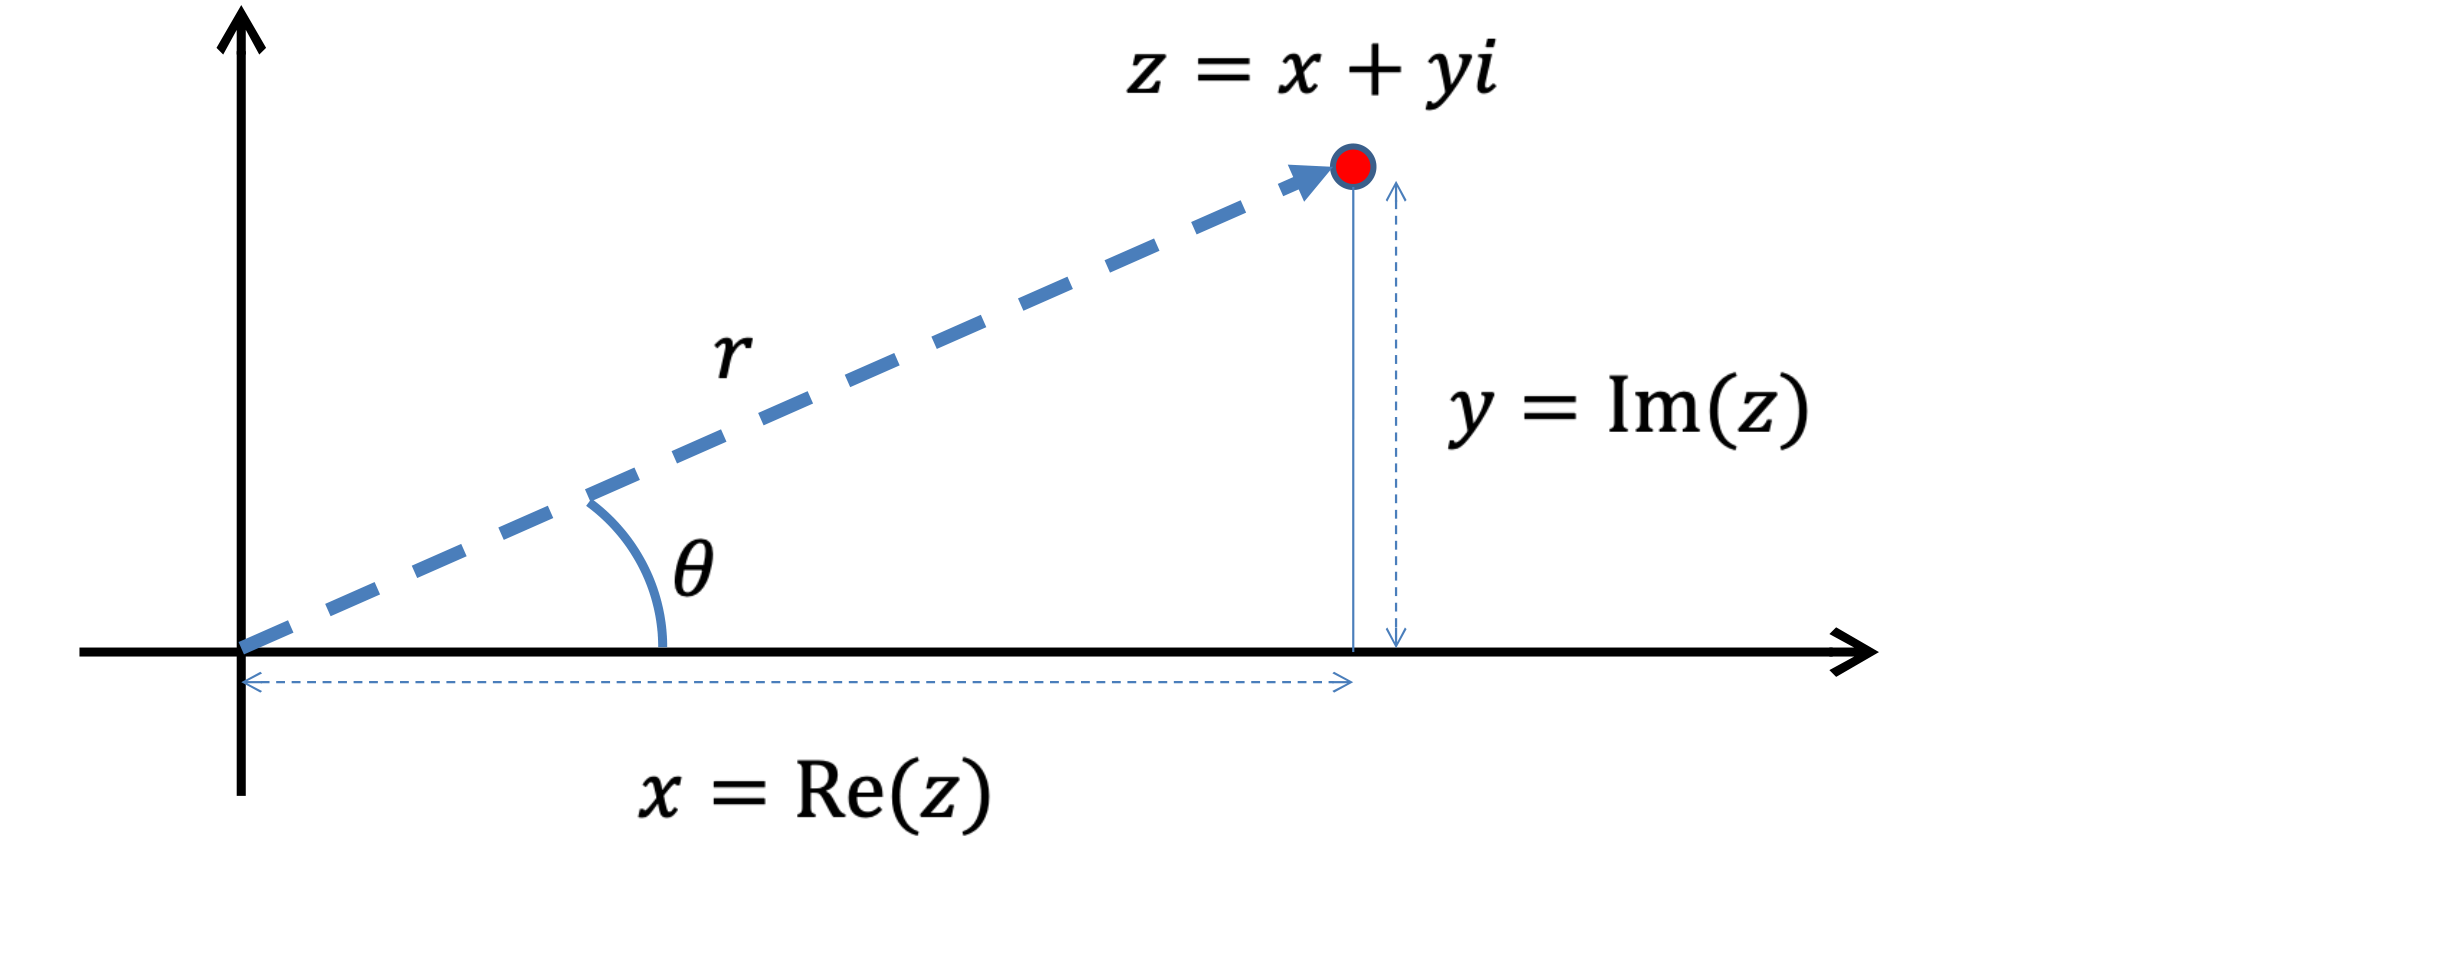
\includegraphics[width=0.7\linewidth]{Figures/Section5/polar_coordinates.png}
    \caption{An Argand diagram where the complex number $z$ is given by its polar coordinates $r$ and $\theta$.}
    \label{fig:polar}
\end{figure}

\begin{example}[DIY]
\label{ex:531}
Write the following complex numbers in standard form. \par
(a) ${z}_{1}$ which has modulus 5 and argument $\frac{\pi }{3}$ \par
(b) ${z}_{2}$ where $\left|{z}_{2}\right|=3$ and $\operatorname{Arg}\left({z}_{2}\right)=\frac{7\pi }{6}$ \par
\end{example}

\begin{blanksol}
(a) Starting from polar form
\begin{align*}
    \quad {z}_{1}&=5\left[\cos \left(\frac{\pi }{3}\right)+i\sin \left(\frac{\pi }{3}\right)\right]\\
    &=5\left(\frac{1}{2}+\frac{\sqrt{3}}{2}i \right) = \frac{5}{2}+\frac{5\sqrt{3}}{2}i \; .
\end{align*}
(b) Again, from polar form
\begin{align*}
\text{(b)}\quad {z}_{2}&=3\left[\cos \left(\frac{7\pi }{6}\right)+i\sin \left(\frac{7\pi }{6}\right)\right]\\
&=3\left(-\frac{\sqrt{3}}{2} - \frac{1}{2}i\right) = -\frac{3\sqrt{3}}{2} - \frac{3}{2}i
\end{align*}
\end{blanksol}

\goodbreak
\begin{example}[Lecture]
\label{ex:532}
Convert the following complex numbers from standard to polar form.
(a) ${z}_{1}=2+2i$ \qquad \qquad (b) ${z}_{2}=-\sqrt{3}-i$
\end{example}
\begin{solution}
(a) Write ${z}_{1}={r}_{1}\left(\cos {\theta }_{1}+i\sin {\theta }_{1}\right)$ then ${r}_{1}=\blank{\left|{z}_{1}\right|=\sqrt{{2}^{2}+{2}^{2}}=\sqrt{8}=2\sqrt{2}}$.\par
${z}_{1}$ is in the \blankpar{first} quadrant, so ${\theta }_{1}=\blank{{\tan }^{-1}\left(\frac{2}{2}\right)=\frac{\pi }{4}}$ therefore 
\[
{z}_{1}=\blank{2\sqrt{2}\left(\cos \frac{\pi }{4}+i\sin \frac{\pi }{4}\right)} \qquad {\rm for} \; 0\leq \theta \leq 2\pi \; .
\]

(b) Write ${z}_{2}={r}_{2}\left(\cos {\theta }_{2}+i\sin {\theta }_{2}\right)$ then ${r}_{2}=\blank{\left|{z}_{2}\right|=\sqrt{3+{1}^{2}}=2}$. \par
${z}_{2}$ is in the\blankpar{ third }quadrant, so ${\theta }_{2}=\blank{{\tan }^{-1}\left(\frac{1}{\sqrt{3}}\right)+\pi =\frac{7\pi }{6}}$, therefore
\[
{z}_{2}=\blank{2\left(\cos \frac{7\pi }{6}+i\sin \frac{7\pi }{6}\right)} \qquad {\rm for} \; 0\leq \theta \leq 2\pi \; .
\]
\end{solution}

\textbf{Multiplication and Division in Polar Form.} Consider the two complex numbers ${z}_{1}={r}_{1}\left(\cos {\theta }_{1}+i\sin {\theta }_{1}\right)$ ${z}_{2}={r}_{2}\left(\cos {\theta }_{2}+i\sin {\theta }_{2}\right)$. Multiplying them together gives
\begin{align*}
{z}_{1}{z}_{2} & ={r}_{1}{r}_{2}\left(\cos {\theta }_{1}+i\sin {\theta }_{1}\right)\left(\cos {\theta }_{2}+i\sin {\theta }_{2}\right)
\\[4pt]
&={r}_{1}{r}_{2}\left(\cos {\theta }_{1}\cos {\theta }_{2}+i\sin {\theta }_{1}\cos {\theta }_{2}+i\cos {\theta }_{1}\sin {\theta }_{2}+{i}^{2}\sin {\theta }_{1}\sin {\theta }_{2}\right)
\\[4pt]
&={r}_{1}{r}_{2}\left[\left(\cos {\theta }_{1}\cos {\theta }_{2}-\sin {\theta }_{1}\sin {\theta }_{2}\right)+i\left(\sin {\theta }_{1}\cos {\theta }_{2}+\cos {\theta }_{1}\sin {\theta }_{2}\right)\right]
\\[4pt]
&={r}_{1}{r}_{2}\left[\cos \left({\theta }_{1}+{\theta }_{2}\right)+i\sin \left({\theta }_{1}+{\theta }_{2}\right)\right] \; .
\end{align*}
Therefore, 
\begin{align}
\label{eq:polar_mult} {z}_{1}{z}_{2}={r}_{1}{r}_{2}\left[\cos \left({\theta }_{1}+{\theta }_{2}\right)+i\sin \left({\theta }_{1}+{\theta }_{2}\right)\right] \; ,
\end{align}
and
\begin{align}
\frac{{z}_{1}}{{z}_{2}}=\frac{{r}_{1}}{{r}_{2}}\left[\cos \left({\theta }_{1}-{\theta }_{2}\right)+i\sin \left({\theta }_{1}-{\theta }_{2}\right)\right] \; .
\end{align}
\textit{I.e.} to multiply two complex numbers, multiply their moduli and add their arguments. To divide them, divide their moduli and subtract the argument of the denominator from the argument of the numerator.

\goodbreak
\begin{example}[Lecture]
\label{ex:533}
Convert ${z}_{1}=-2+2\sqrt{3}i$ and ${z}_{2}=5-5i$ to polar form. Hence, find ${z}_{1}{z}_{2}$ and $\frac{{z}_{1}}{{z}_{2}}$.
\end{example}
%
\begin{solution}
Write ${z}_{1}={r}_{1}\left(\cos {\theta }_{1}+i\sin {\theta }_{1}\right)$ and ${z}_{2}={r}_{2}\left(\cos {\theta }_{2}+i\sin {\theta }_{2}\right)$ where ${r}_{1}=\blank{\sqrt{4+12}=4}$ and ${r}_{2}=\blank{\sqrt{25+25}=5\sqrt{2}}$. 

The argument ${\theta }_{1}$ is in the second quadrant, so ${\theta }_{1}=\blank{{\tan }^{-1} \left(-\sqrt{3}\right) + \pi =\frac{2\pi }{3}}$. The argument ${\theta }_{2}$ is in the fourth quadrant, so ${\theta }_{1}=\blank{{\tan }^{-1} \left(-1\right) = -\frac{\pi}{4}} \qquad {\rm or} \qquad \blank{\frac{7\pi }{4}}$.

% Main deck slide 35

So, 
\[
{z}_{1}=\blank{4\left(\cos \frac{2\pi }{3}+i\sin \frac{2\pi }{3}\right)} \qquad {\rm and} \qquad {z}_{2}=\blank{5\sqrt{2}\left(\cos \frac{7\pi }{4}+i\sin \frac{7\pi }{4}\right)}
\]
Then, multiplying the moduli and adding the arguments we find
\[
{z}_{1}{z}_{2}=\blank{20\sqrt{2}\left[\cos \left(\frac{29\pi }{12}\right)+i\sin \left(\frac{29\pi }{12}\right)\right]} =\blank{20\sqrt{2}\left(\cos \frac{5\pi }{12}+i\sin \frac{5\pi }{12}\right)} \; .
\]
Dividing the moduli and subtracting the arguments we find
\[
\frac{{z}_{1}}{{z}_{2}}=\blank{\frac{2\sqrt{2}}{5}\left[\cos \left(\frac{-13\pi }{12}\right)+i\sin \left(\frac{-13\pi }{12}\right)\right]} = \blank{\frac{2\sqrt{2}}{5}\left[\cos \frac{11\pi }{12}+i\sin \frac{11\pi }{12}\right]} \; .
\]
\end{solution}

\goodbreak
\textbf{Powers in Polar Form.} It follows from equation \eqref{eq:polar_mult} that if we raise the complex number $z=r\left(\cos \theta +i\sin \theta \right)$ to the power $n$, we get
\begin{align}
{z}^{n}={r}^{n}\left[\cos \left(n\theta \right)+i\sin \left(n\theta \right)\right] \; .
\end{align}
\textit{I.e.} raise the modulus to the power $n$ and multiply the argument by $n$. This is known as \textbf{De Moivre’s theorem}. This is visualised in the animation in figure \ref{anim:argand_power}.
\begin{figure}[ht]
    \iflatexml
        \<div id="argand-power-widget">\</div> 
        % \<script src="bmluser/argand-power-plotly-bookml.js">\</script>
        \caption{Interactive plot of the complex numbers $z$ (blue) and $z^n$ (red) on an Argand diagram, where the modulus and argument of $z$ and the power $n$ can be altered with the sliders.}
    \else
    \centering
    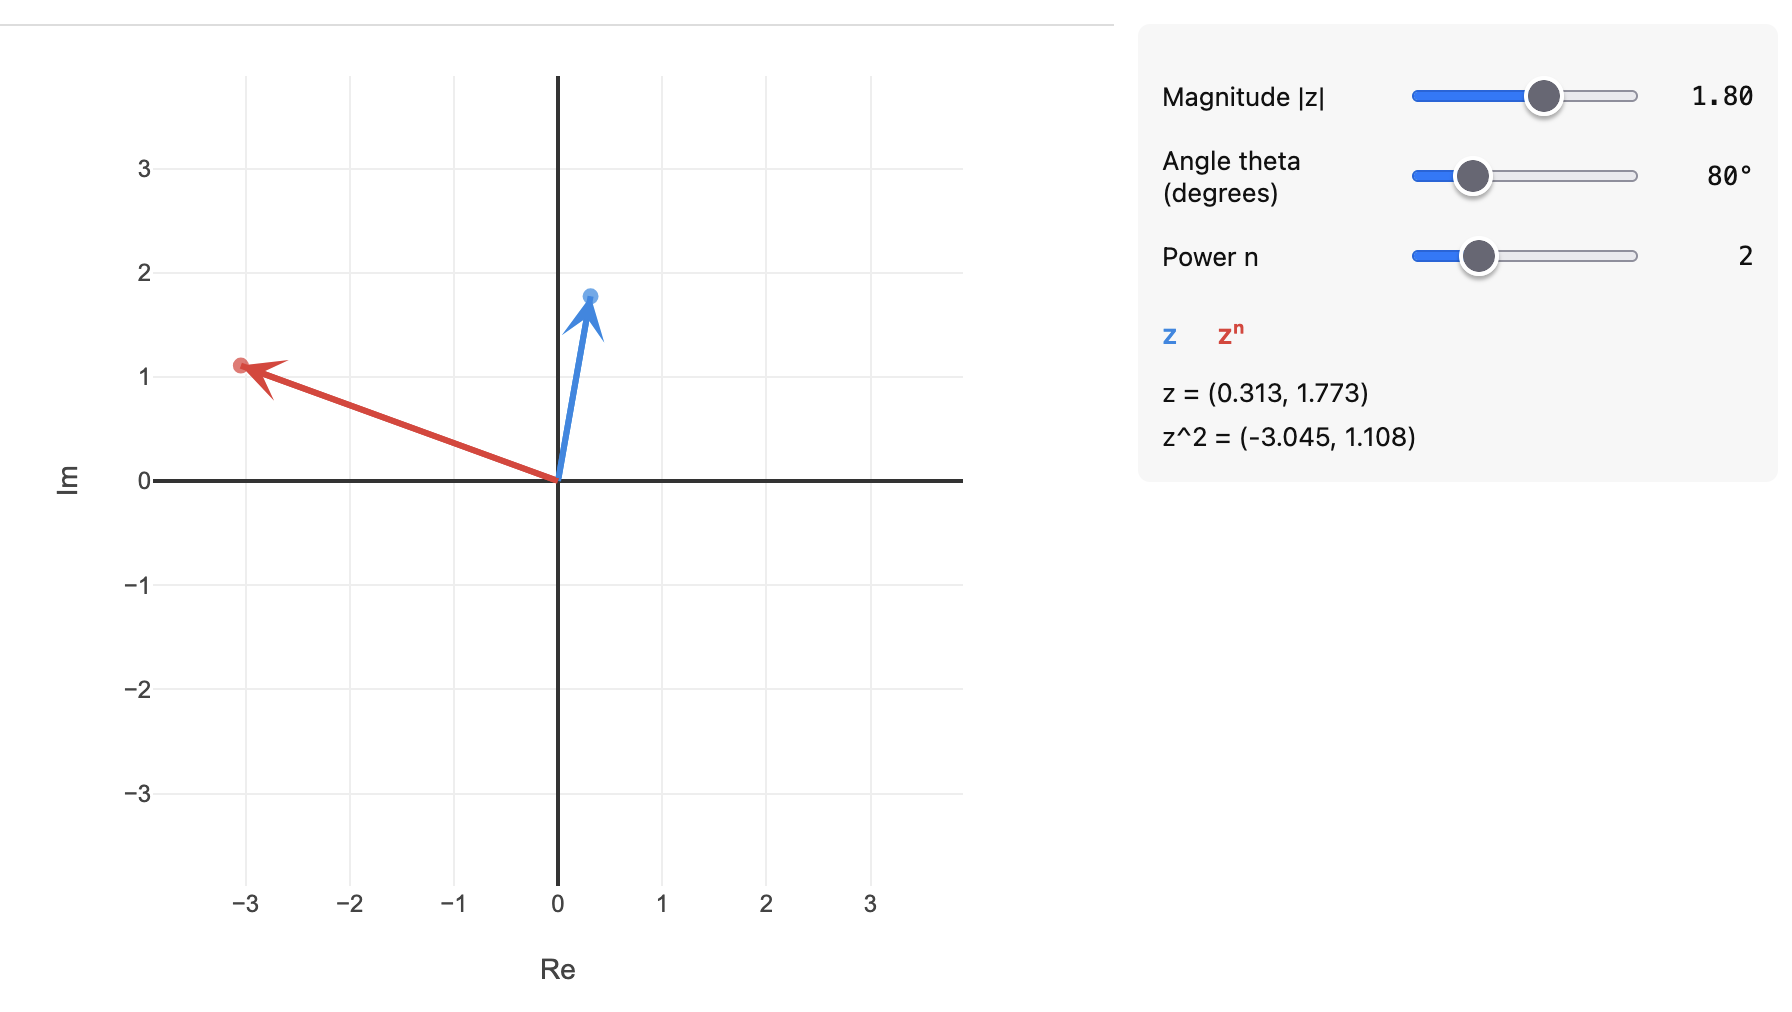
\includegraphics[width=0.8\textwidth]{Figures/Section5/screenshot_argand_power.png}
    \caption{Screenshot of the interactive plot of the complex numbers $z$ (blue) and $z^n$ (red) on an Argand diagram (available in the HTML version of these notes).}
    \fi
    \label{anim:argand_power}
\end{figure}

\textbf{The Exponential Form.} Note that this polar form can be written in an alternative manner
\begin{align}
r\left(\cos \theta +i\sin \theta \right)\equiv r{e}^{i\theta } \;. 
\end{align}
This is known as \textbf{Euler’s formula}. For the special case $r=1$ and $\theta =\pi $, we see
\[
{e}^{i\pi }=-1 \; ,
\]
Also known as Euler’s identity, often written ${e}^{i\pi }+1=0$. This equation elegantly links some of the most fundamental mathematical constants $e$, $i$, $\pi$, and $-1$. 

It follows that, if ${z}_{1}={r}_{1}{e}^{i{\theta }_{1}}$ and ${z}_{2}={r}_{2}{e}^{i{\theta }_{2}}$ then
\begin{align*}
{z}_{1}{z}_{2} & ={r}_{1}{r}_{2}{e}^{i\left({\theta }_{1}+{\theta }_{2}\right)}
\\[4pt]
\frac{{z}_{1}}{{z}_{2}} &= \frac{{r}_{1}}{{r}_{2}}{e}^{i\left({\theta }_{1}-{\theta }_{2}\right)}
\\[4pt]
{z}_{1}^{n} &={r}_{1}^{n}{e}^{in{\theta }_{1}}
\end{align*}
Therefore, under these basic arithmetic operations, the complex exponential behaves the same as the exponential of real numbers.

\goodbreak
\begin{example}[DIY]
\label{ex:534}
Find
\[
{\left(-\frac{1}{\sqrt{2}}+\frac{i}{\sqrt{2}}\right)}^{17}
\]
and express in the form $x+yi$.
\end{example}
%
\begin{blanksol}
If $z=\left(-\frac{1}{\sqrt{2}}+\frac{i}{\sqrt{2}}\right)$ then $\left|z\right|=\sqrt{\frac{1}{2}+\frac{1}{2}}=1$ and $\operatorname{Arg}\left(z\right)={\tan }^{-1} (-1) + \pi =\frac{3\pi }{4}$. So, $z=\exp \left(i\frac{3\pi }{4}\right)$ therefore

\begin{align*}
{z}^{17}&=\exp \left(i\frac{51\pi }{4}\right) =\exp \left[i\left(12\pi +\frac{3\pi }{4}\right)\right]\\
&=\exp \left(i\frac{3\pi }{4}\right) =-\frac{1}{\sqrt{2}}+\frac{i}{\sqrt{2}}
\end{align*}
\end{blanksol}

\goodbreak
\begin{example}[Video]
\label{ex:535}
Use De Moivre’s theorem to find an identity for $\cos 4\theta $ in terms of $\cos \theta $ and $\sin \theta $.
\end{example}

\begin{solution}
Defining $z=\left(\cos \theta +i\sin \theta \right)$, then from De Moivre’s theorem for $n=4$
\[
{z}^{4}=\left[\cos \left(4\theta \right)+i\sin \left(4\theta \right)\right]
\]
Using direct multiplication
\[
{z}^{2}=z\times z=\blank{{\cos }^{2} \theta -{\sin }^{2} \theta +2i\sin \left(\theta \right)\cos \left(\theta \right)} \equiv \blank{a+bi}
\]
and again
\[
{z}^{4}={z}^{2}\times {z}^{2}=\blank{{a}^{2}-{b}^{2}+2iab}
\]
Comparing real parts of both sides $\operatorname{Re}\left({z}^{4}\right)={a}^{2}-{b}^{2}$. Then, using the expression from De Moivre’s theorem
\begin{align*}
\cos \left(4\theta \right) &=\blank{{\left({\cos }^{2} \theta -{\sin }^{2} \theta \right)}^{2}-4{\sin }^{2} \left(\theta \right){\cos }^{2} \left(\theta \right)}
\\[4pt]
\therefore \cos \left(4\theta \right) &=\blank{{\cos }^{4} \theta -6{\sin }^{2} \left(\theta \right){\cos }^{2} \left(\theta \right)+{\sin }^{4} \theta \; .}
\end{align*}
\end{solution}


\goodbreak
\begin{recap}{\ref{sec:complex_polar}}

\item Polar and exponential forms express a complex number in terms of its modulus and argument

\[
x+iy\equiv r\left(\cos \theta +i\sin \theta \right)\equiv r{e}^{i\theta }
\]

\item Multiplication, division and powers of complex numbers are simpler to calculate in these forms e.g.

\[
\begin{aligned}
{z}_{1}{z}_{2}&={r}_{1}{r}_{2}{e}^{i\left({\theta }_{1}+{\theta }_{2}\right)} \frac{{z}_{1}}{{z}_{2}}\\
&=\frac{{r}_{1}}{{r}_{2}}{e}^{i\left({\theta }_{1}-{\theta }_{2}\right)} {z}_{1}^{n}\\
&={r}_{1}^{n}{e}^{in{\theta }_{1}}
\end{aligned}
\]
\end{recap}

\newtexpage
\subsection{Complex Roots}
\label{sec:complex_roots}

\begin{learningoutcomes}
\item Find all the complex roots of a monomial or polynomial equation
\item Plot the roots of a complex number on an Argand diagram
\end{learningoutcomes}

% Main deck slide 44

\textbf{Roots of Complex Numbers.} Consider the equation
\[
{z}^{2}=64
\]
This equation has two solutions i.e. $z=8$ and $z=-8$. Now consider the equation
\[
{z}^{3}=64
\]
One solution is $z=4$, but it is a cubic so there are two more solutions $z=-2+2\sqrt{3}i$ and $z=-2-2\sqrt{3}i$.

The solutions to ${z}^{3}=64$ are equally spaced around a circle. ${z}_{1}=4$, ${z}_{2}=-2+2\sqrt{3}i$ and ${z}_{3}=-2-2\sqrt{3}i$, see figure \ref{fig:cube_roots}(a).
\begin{figure}
    \centering
    \subfig{0.48}{Figures/Section5/cube_roots_64.png}{}
    \subfig{0.48}{Figures/Section5/fourth_roots_1_plus_i.png}{}
    \caption{(a) The roots of the equation $z^3=64$ on an Argand diagram are equally spaced around the circle of radius 4 centred at the origin. (b) The roots of the equation $z^4=1+i$ on an Argand diagram.}
    \label{fig:cube_roots}
\end{figure}

In general, the equation
\[
{z}^{n}=a+bi
\]
will have $n$ solutions that are spaced equally around a circle in the Argand Diagram. For example, the roots of the equation ${z}^{4}=1+i$ are plotted in \ref{fig:cube_roots}(b).

To find the solutions of ${z}^{n}=a+bi$ first express $a+bi $ in exponential form \textit{i.e.}
\[
a + bi = r{e}^{i\theta } \; .
\]
Now, note that $2\pi$ can be added to the argument without changing the complex number itself $a+bi=r{e}^{i\theta }=$ $r{e}^{i(\theta +2\pi )}$ = $r{e}^{i(\theta +4\pi )}=\ldots =r{e}^{i(\theta +2(n-1)\pi )}$. This gives $n$ different, but equivalent arguments. Dividing these by $n$ gives all the roots for $0\leq \theta \leq 2\pi $. 

% Main deck slide 48
Returning to ${z}^{3}=64$, we can rewrite as ${z}^{3}=64{e}^{0i}$ and furthermore as
\[
{z}^{3}=64{e}^{0i}=64{e}^{2\pi i}=64{e}^{4\pi i} \; .
\]
Taking the cube root, the modulus is the real root of $\sqrt[3]{64}=4$, and the argument is divided by 3, resulting in the three solutions 
\[{z}_{1}=4{e}^{0i} \qquad \qquad {z}_{2}=4{e}^{\frac{2\pi i}{3}} \qquad \qquad {z}_{3}=4{e}^{\frac{4\pi i}{3}} \; .\]
Converting back to standard form
\begin{align*}
{z}_{1} &=4 \\[4pt]
{z}_{2}&=4\left[\cos \left(\frac{2\pi }{3}\right)+i\sin \left(\frac{2\pi }{3}\right)\right]\\
&=4\left(-\frac{1}{2}+\frac{\sqrt{3}}{2}i\right) =-2+2\sqrt{3}i \\[4pt]
{z}_{3}&=4\left[\cos \left(\frac{4\pi }{3}\right)+i\sin \left(\frac{4\pi }{3}\right)\right]\\
&=4\left(-\frac{1}{2}-\frac{\sqrt{3}}{2}i\right) = -2-2\sqrt{3}i
\end{align*}
As shown in figure \ref{fig:cube_roots}, the solutions are equally spaced around a circle. ${z}_{1}=4$, ${z}_{2}=-2+2\sqrt{3}i$ and ${z}_{3}=-2-2\sqrt{3}i$ ${z}_{1}=4{e}^{i0}$, ${z}_{2}=4{e}^{\frac{i2\pi }{3}}$ and ${z}_{3}=4{e}^{-\frac{i2\pi }{3}}$.

\goodbreak
\begin{example}[Lecture]
\label{ex:541}
Find all solutions to the equation
\[
{z}^{4}=-9
\]
Give your answers in the form $z=a+bi$.
\end{example}

\begin{solution}
In exponential form $-9=\blank{9{e}^{i\pi }}$, incrementing the argument by $2\pi $
\[
{z}^{4}=\blank{9{e}^{i\pi } }=\blank{9{e}^{i3\pi } }=\blank{9{e}^{i5\pi } }=\blank{9{e}^{i7\pi }}
\]
The modulus of the roots is $\blank{\sqrt[4]{9}=\sqrt{3}}$ and so the roots are \begin{align*}
{z}_{1}&=\blank{\sqrt{3}{e}^{\frac{i\pi }{4}}} \, , \qquad {z}_{2}=\blank{\sqrt{3}{e}^{\frac{i3\pi }{4}}} \, ,\\[4pt]
\qquad {z}_{3}&=\blank{\sqrt{3}{e}^{\frac{i5\pi }{4}}}\, , \qquad {z}_{4}=\blank{\sqrt{3}{e}^{\frac{i7\pi }{4}}} \, .
\end{align*}
Converting to standard form
\begin{align*}
{z}_{1}&= \blank{\sqrt{3}\left(\cos \frac{\pi }{4}+i\sin \frac{\pi }{4}\right) } =\blank{\sqrt{\frac{3}{2}}+\sqrt{\frac{3}{2}}i}\, , \\[4pt]
%
{z}_{2}&= \blank{\sqrt{3}\left(\cos \frac{3\pi }{4}+i\sin \frac{3\pi }{4}\right)} =\blank{-\sqrt{\frac{3}{2}}+\sqrt{\frac{3}{2}}i}\, ,\\[4pt]
%
{z}_{3}&= \blank{\sqrt{3}\left(\cos \frac{5\pi }{4}+i\sin \frac{5\pi }{4}\right)} =\blank{-\sqrt{\frac{3}{2}}-\sqrt{\frac{3}{2}}i} \, ,\\[4pt]
%
{z}_{4}&= \blank{\sqrt{3}\left(\cos \frac{7\pi }{4}+i\sin \frac{7\pi }{4}\right)} =\blank{\sqrt{\frac{3}{2}}-\sqrt{\frac{3}{2}}i} \, .
\end{align*}

\ifcsname insertBlanks\endcsname
\else
\begin{center}
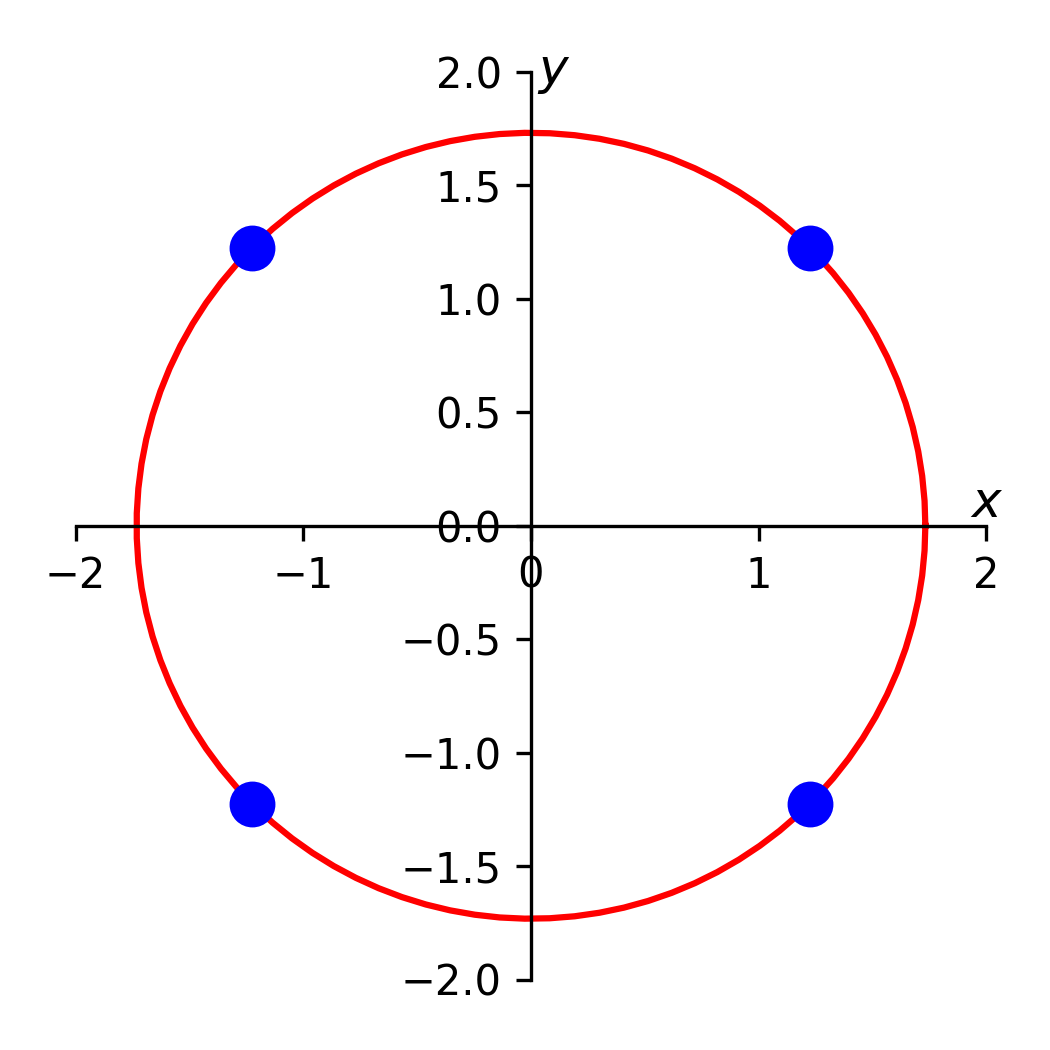
\includegraphics[width=.4\linewidth]{Figures/Section5/fourth_roots_minus_9.png}
\end{center}
\fi
\end{solution}

% Main deck slide 53

\textbf{Roots of Polynomial Equations.} An $n$-th degree polynomial equation can have up to $n$ real roots, some of which may be repeated. Including complex roots, an $n$-th degree polynomial equation will always have $n$ solutions  (including repeated roots). \textit{E.g.}
\[
{z}^{3}+{z}^{2}-7z-15=0
\]
has solutions $z=3$, $z=-2+i$, and $z=-2-i$.

Recall the example with no real roots from the start of this section
\[
f\left(z\right)={z}^{2}-8z+17=0 \; .
\]
The complex roots are where both the real and imaginary parts of $f\left(z\right)$ are 0 (see figure \ref{fig:poly_roots}).
\begin{figure}
    \centering
    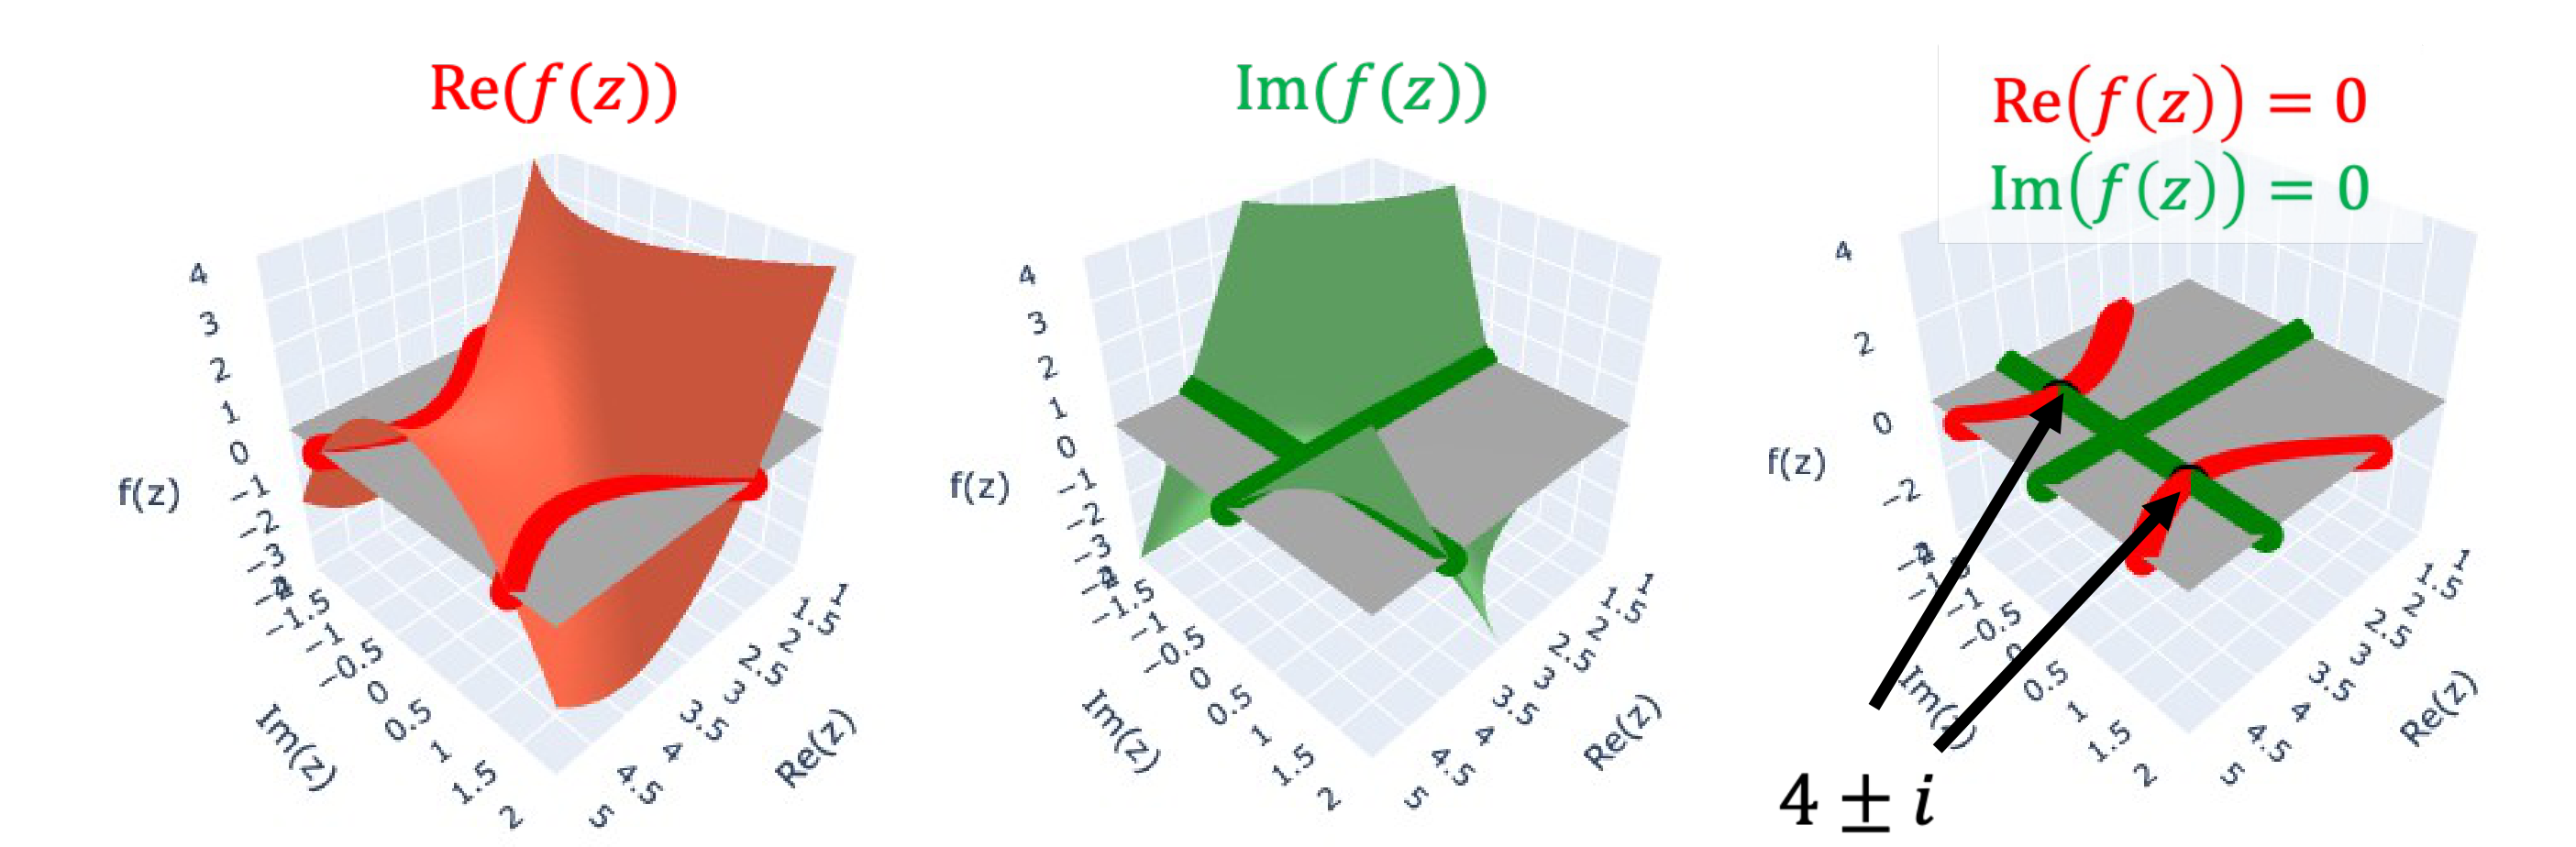
\includegraphics[width=0.9\linewidth]{Figures/Section5/complex_polynomial_surfaces.png}
    \caption{Visualisation of the complex roots of $f(z) \equiv {z}^{2}-8z+17=0$ where the $x$ and $y$ axes are the real and imaginary parts of $z$ respectively and the grey plane corresponds to $f(z)=0$. Left: The red surface shows the real value of $f(z)$. Middle: The green surface shows the imaginary values of $f(z)$. Right: The green and red lines show where the real and imaginary parts of $f(z)$ are zero, respectively. Where these lines cross are the roots of the equation.}
    \label{fig:poly_roots}
\end{figure}

If $z=a+bi$ is a solution to a polynomial equation with real coefficients, then so is the conjugate $\overline{z}=a-bi$. It follows that $z-a-bi$ and $z-a+bi$ will be factors of the polynomial and so
\begin{align*}
    \left(z-a-bi\right)\left(z-a+bi\right)&={\left(z-a\right)}^{2}+{b}^{2} \\[4pt]
    &={z}^{2}-2az+{a}^{2}+{b}^{2} \; ,
\end{align*}
is a factor of the polynomial.

% Main deck slide 56

\goodbreak
\begin{example}[Lecture]
\label{ex:542}
Given that $z=1+i$ is a solution to the equation
\[
{z}^{3}+2{z}^{2}-6z+8=0
\]
find the other solutions.
\end{example}

\begin{solution}
The cubic equation has real coefficients, so $z=\blank{1-i}$ must also be a solution. Thus, we can factorise the cubic as
\begin{align*}
{z}^{3}+2{z}^{2}-6z+8 &= \blank{\left(z-1-i\right)\left(z-1+i\right)\left(z-c\right)} \\
&=\blank{\left({z}^{2}-2z+2\right)\left(z-c\right)}\\
&=\blank{{z}^{3}-\left(2+c\right){z}^{2}+2\left(1+c\right)z-2c}
\end{align*}
Comparing coefficients, we see the final root is $z=\blank{c=-4}$.
\end{solution}

\goodbreak
\begin{example}[Video]
\label{ex:543}
Find the complex values of $z$ that satisfy the equation
\[
{z}^{2}+\left(2+4i\right)z-3+\frac{7}{4}i=0
\]
\end{example}

\begin{solution}
Use the quadratic equation (or discriminant method)
\[
z=-\frac{b}{2}+\frac{1}{2}{\left({b}^{2}-4c\right)}^{\frac{1}{2}}
\]
with $b=\blank{2+4i}$ and $c=-\blank{3+\frac{7}{4}i}$. This gives
\begin{align*}
    z &=\blank{-1-2i+\frac{1}{2}{\left(4+16i+16{i}^{2}+12-7i\right)}^{\frac{1}{2}}} \\[4pt]
    &= \blank{-1-2i+\frac{1}{2}{\left(9i\right)}^{\frac{1}{2}}}
\end{align*}
Let $w=\blank{9i}$, in exponential form $w=\blank{9{e}^{\frac{i\pi }{2}}} =\blank{9{e}^{\frac{i5\pi }{2}}}$. Then 
\begin{align*}
{w}^{\frac{1}{2}} &=\blank{3{e}^{\frac{i\pi }{4}}} =\blank{\frac{3}{\sqrt{2}}(1+i)} \\
&{\rm or} \\
{w}^{\frac{1}{2}}&=\blank{3{e}^{\frac{i5\pi }{4}}} =\blank{-\frac{3}{\sqrt{2}}(1+i)} \; .
\end{align*}

So, $\displaystyle z=\blank{\left(-1+\frac{3\sqrt{2}}{4}\right)+\left(-2+\frac{3\sqrt{2}}{4}\right)i}$ \\
or \\
$\displaystyle z=\blank{\left(-1-\frac{3\sqrt{2}}{4}\right)+\left(-2-\frac{3\sqrt{2}}{4}\right)i}$.
\end{solution}

\goodbreak
\begin{recap}{\ref{sec:complex_roots}}
\item A complex (or real) number to the power $1/n$ has $n$ roots
\item To find the roots, generate $n$ equivalent complex numbers by adding $2\pi $ to the argument $n-1$ times
$a+bi=r{e}^{i\theta }=$ $r{e}^{i(\theta +2\pi )}$ = $r{e}^{i(\theta +4\pi )}=\ldots =r{e}^{i(\theta +2(n-1)\pi )}$
\item An $n$-th order polynomial also has $n$ roots (some may be repeated)
\item If the polynomial has real coefficients, then any complex roots $z=a+bi$ will occur in a pair with its conjugate $z=a-bi$
\end{recap}

\subsection{Complex Numbers and Loci}
\label{sec:complex_loci}

\begin{learningoutcomes}
\item Sketch loci in an Argand diagram based on equations or inequalities involving complex numbers.
\end{learningoutcomes}

An equation (or inequality) involving a complex number $z=x+yi$ can be an efficient way to represent a line, curve or area in $x$-$y$ space. Writing in terms of $x$ and $y$ can help to sketch the locus. A reminder of some relationships are given in table \ref{tab:loci}.
\begin{table}[ht]
    \centering
    \begin{tabular}{|c|c|}\hline
         Complex representation & $x$-$y$ representation\\\hline
         $\left|z\right|$ & $\sqrt{{x}^{2}+{y}^{2}}$ \\
         $\operatorname{Re}\left(z\right)$ & $x$ \\
         $\operatorname{Im}\left(z\right)$ & $y$ \\
         $\left|z-w\right|$ & $\sqrt{{(x-a)}^{2}+{(y-b)}^{2}}$\\
         $\operatorname{Re}\left(z-w\right)$ & $x-a$\\
         $\operatorname{Im}\left(z-w\right)$ & $y-b$\\ \hline
    \end{tabular}
    \caption{A list of equivalent expressions in terms of the complex numbers $z=x+yi$ and $w=a+bi$ and in terms $x$, $y$, $a$, and $b$. Note: All of these expressions are real, they do not contain $i$.}
    \label{tab:loci}
\end{table}

Consider the expression $\left|z-w\right|$ which is equivalent to $\sqrt{{(x-a)}^{2}+{(y-b)}^{2}}$, and so can describe loci associated with the circle with centre at $w=(a,b)$. Some relations involving this expression are sketched in figure \ref{fig:circle_loci}.
\begin{figure}
    \centering
    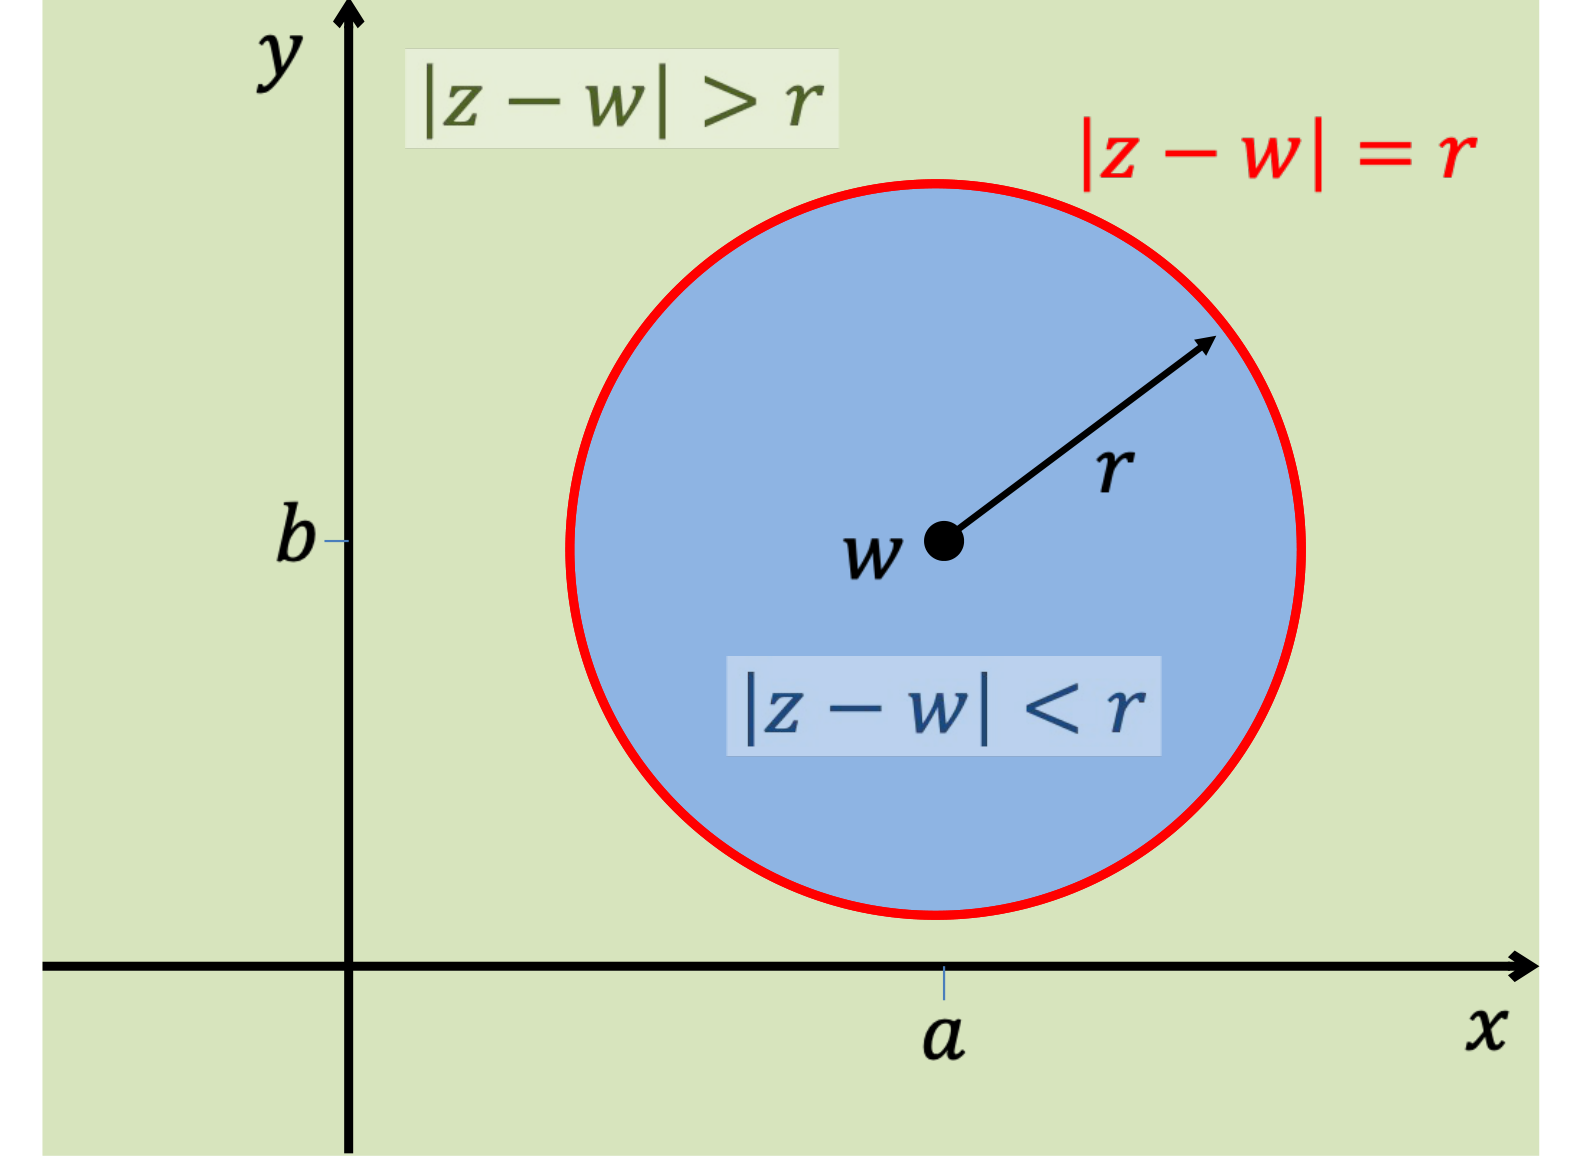
\includegraphics[width=0.6\linewidth]{Figures/Section5/circle_loci.png}
    \caption{A sketch of three loci involving the circle $\left|z-w\right|=r$. When this is an inequality, the locus is all the points inside or outside the circle (blue and green). When it is an equality the locus contains all the points on the circle (red).}
    \label{fig:circle_loci}
\end{figure}

For example, consider the locus given by
\[
2<\left|z\right|\leq 5
\]
It includes all points that are outside the circle ${x}^{2}+{y}^{2}=4$ and inside or on the circle ${x}^{2}+{y}^{2}=25$. This is shown in figure \ref{fig:annulus}.
\begin{figure}
    \centering
    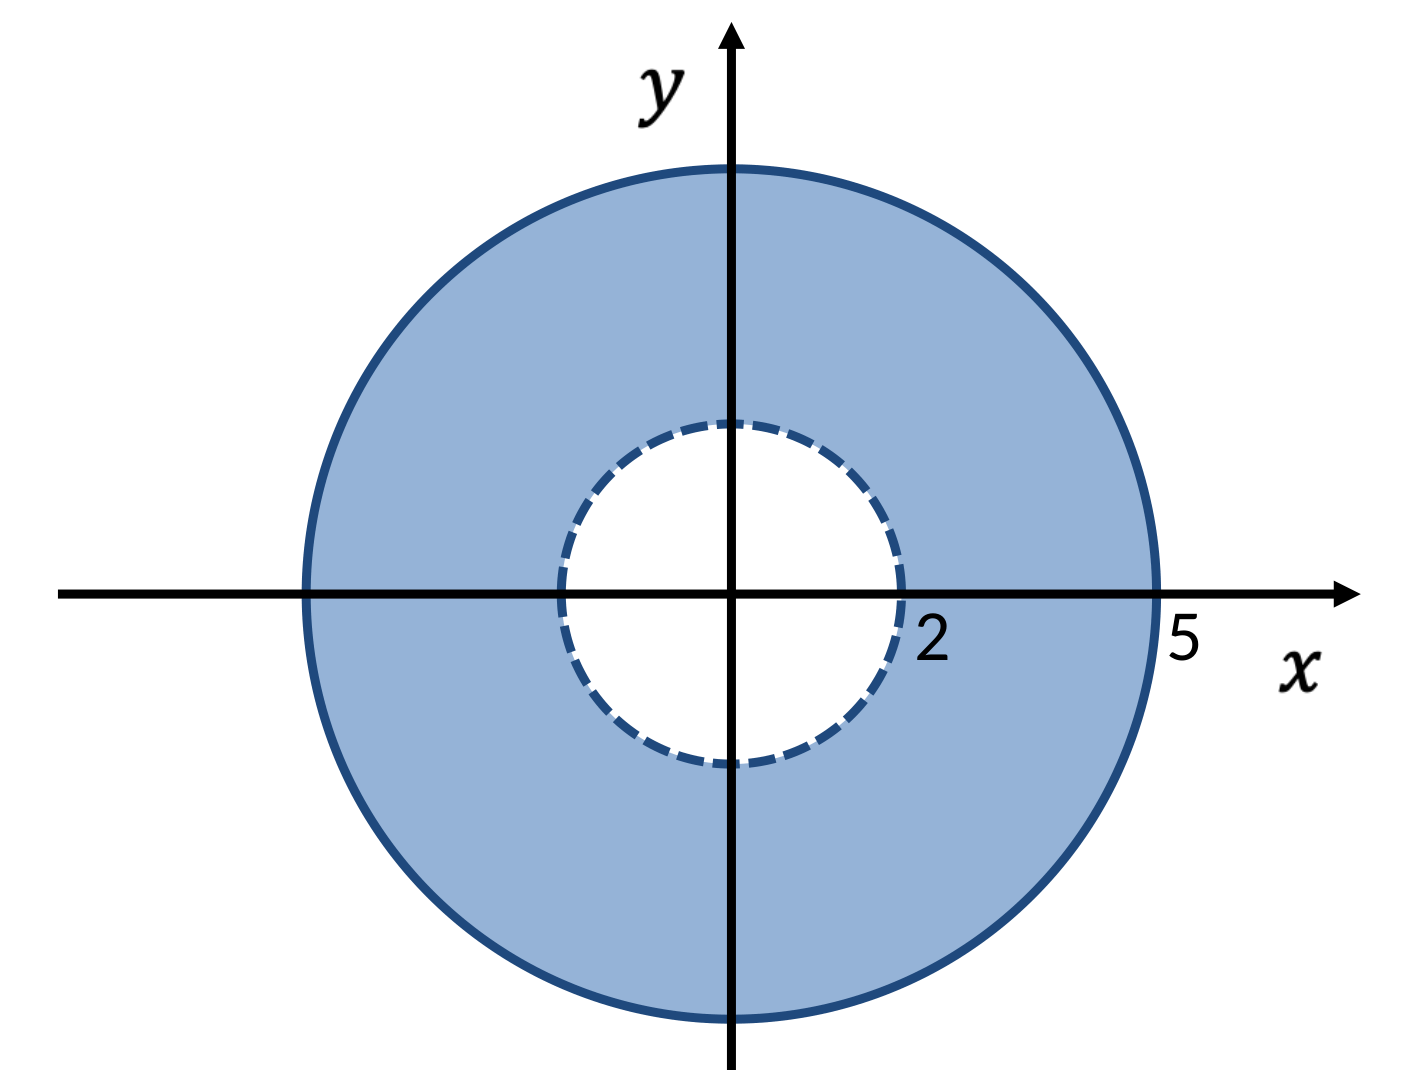
\includegraphics[width=0.55\linewidth]{Figures/Section5/annular_locus.png}
    \caption{The shaded blue region indicates the locus $2<\left|z\right|\leq 5$.}
    \label{fig:annulus}
\end{figure}

\goodbreak
\begin{example}[Lecture]
\label{ex:551}
Find and sketch the loci described by \\[6pt]
(a) $\displaystyle 2\operatorname{Re}\left(z\right)+\operatorname{Im}\left(z-\left(1+2i\right)\right)=10$ \\[6pt]
(b) $\displaystyle \left|z\right|\leq \operatorname{Re}\left(z+2\right)$ \\[6pt]
(c) $\left|z-2+i\right|<3$
\end{example}

\begin{solution}

Express the loci in terms of $x$ and $y$.

(a) $\operatorname{Re}\left(z\right)=\blank{x}$ and $\operatorname{Im}\left(z-\left(1+2i\right)\right)=\blank{y-2}$ so, the locus is 
\[
\blank{2x+y-2=10} \qquad {\rm or} \qquad \blank{y=12-2x} \, .
\]
\ifcsname insertBlanks\endcsname
    \begin{center}
    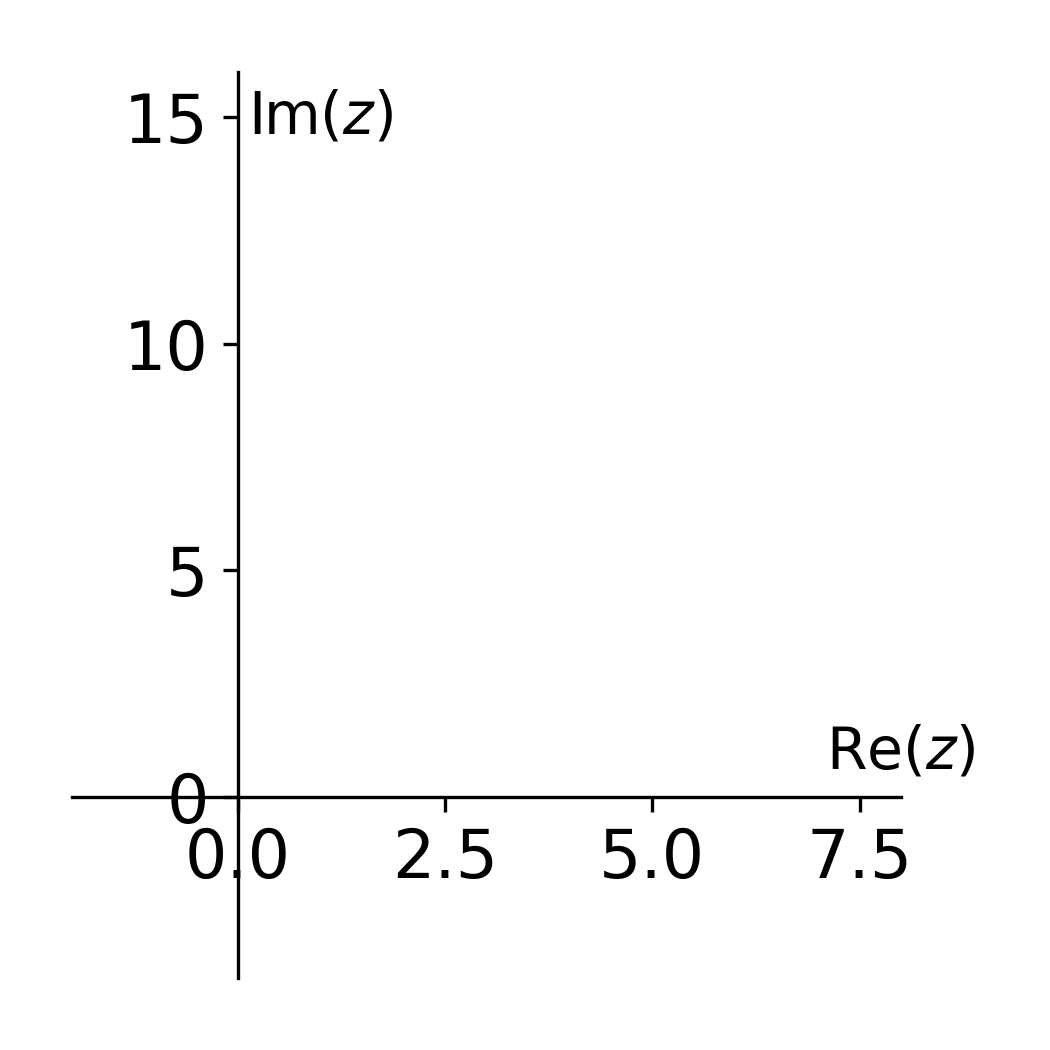
\includegraphics[width=.45\linewidth]{Figures/Section5/loci_ex551a_blank.png}
    \end{center}
\else
    \begin{center}
    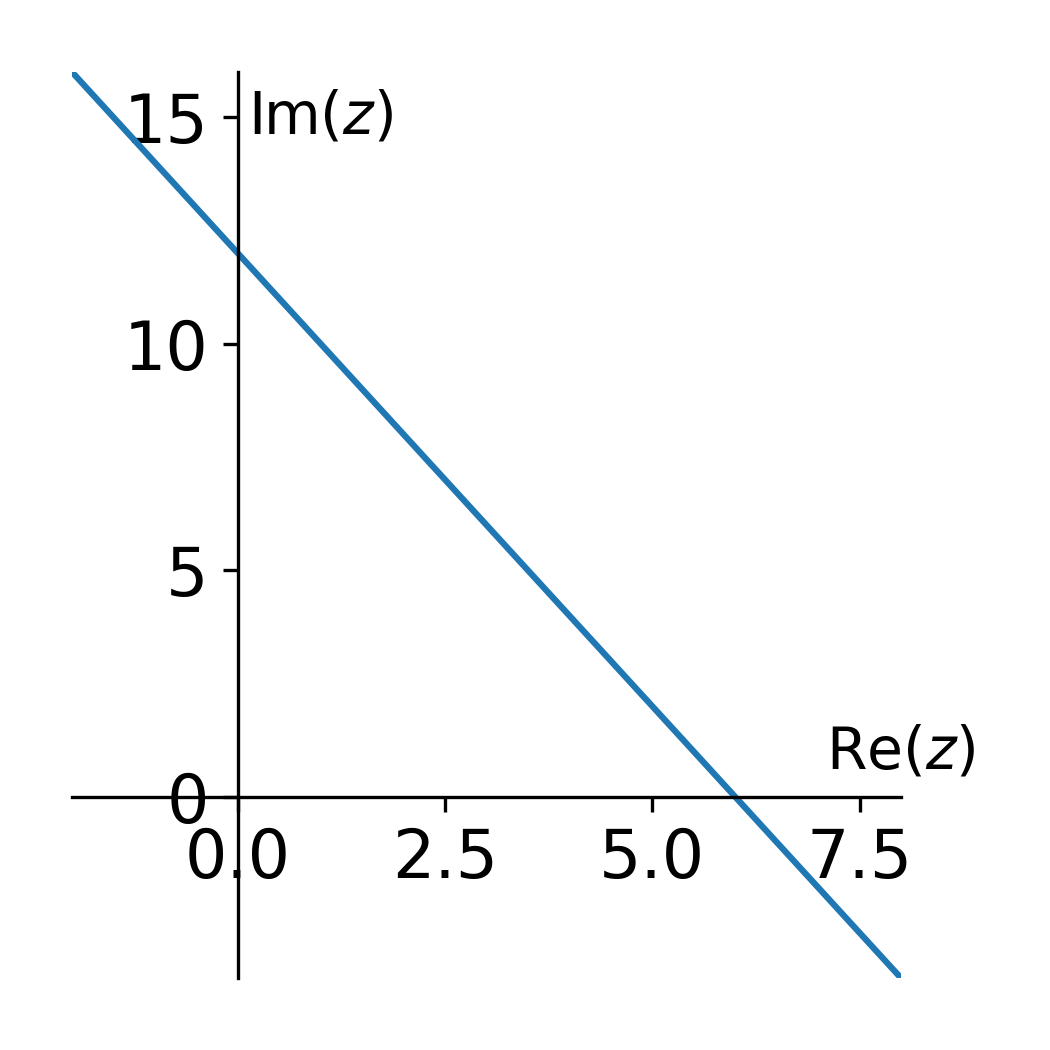
\includegraphics[width=.45\linewidth]{Figures/Section5/loci_ex551a.png}
    \end{center}
\fi

(b) $\left|z\right|=\blank{\sqrt{{x}^{2}+{y}^{2}}}$ and $\operatorname{Re}\left(z+2\right)=\blank{x+2}$ so the locus is 
$\blank{{x}^{2}+{y}^{2}\leq } \blank{{\left(x+2\right)}^{2}}$ or $\blank{{y}^{2}\leq } \blank{4x+4}$ which can be written 
\[
\blank{x\geq \frac{{y}^{2}}{4}-1} \; .
\]
\ifcsname insertBlanks\endcsname
    \begin{center}
    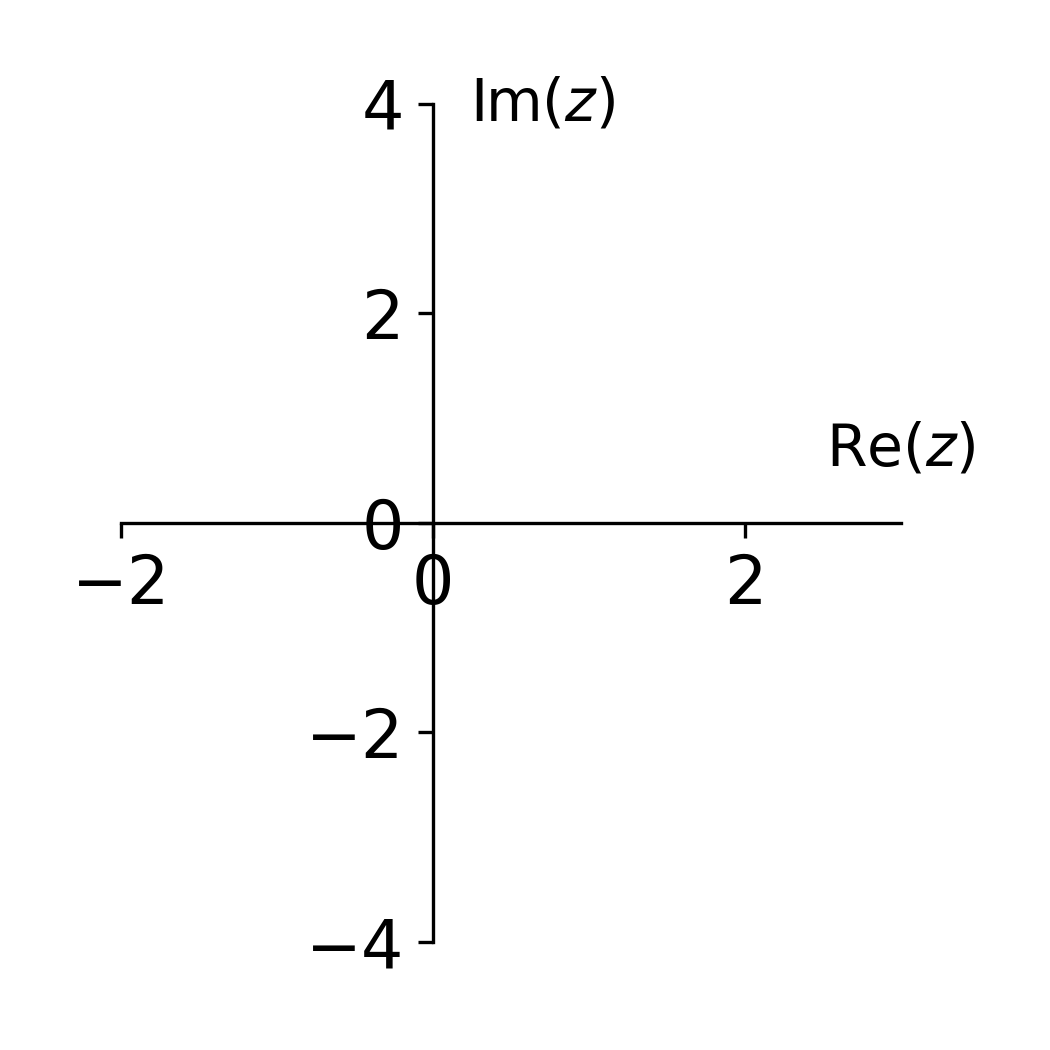
\includegraphics[width=.45\linewidth]{Figures/Section5/loci_ex551b_blank.png}
    \end{center}
\else
    \begin{center}
    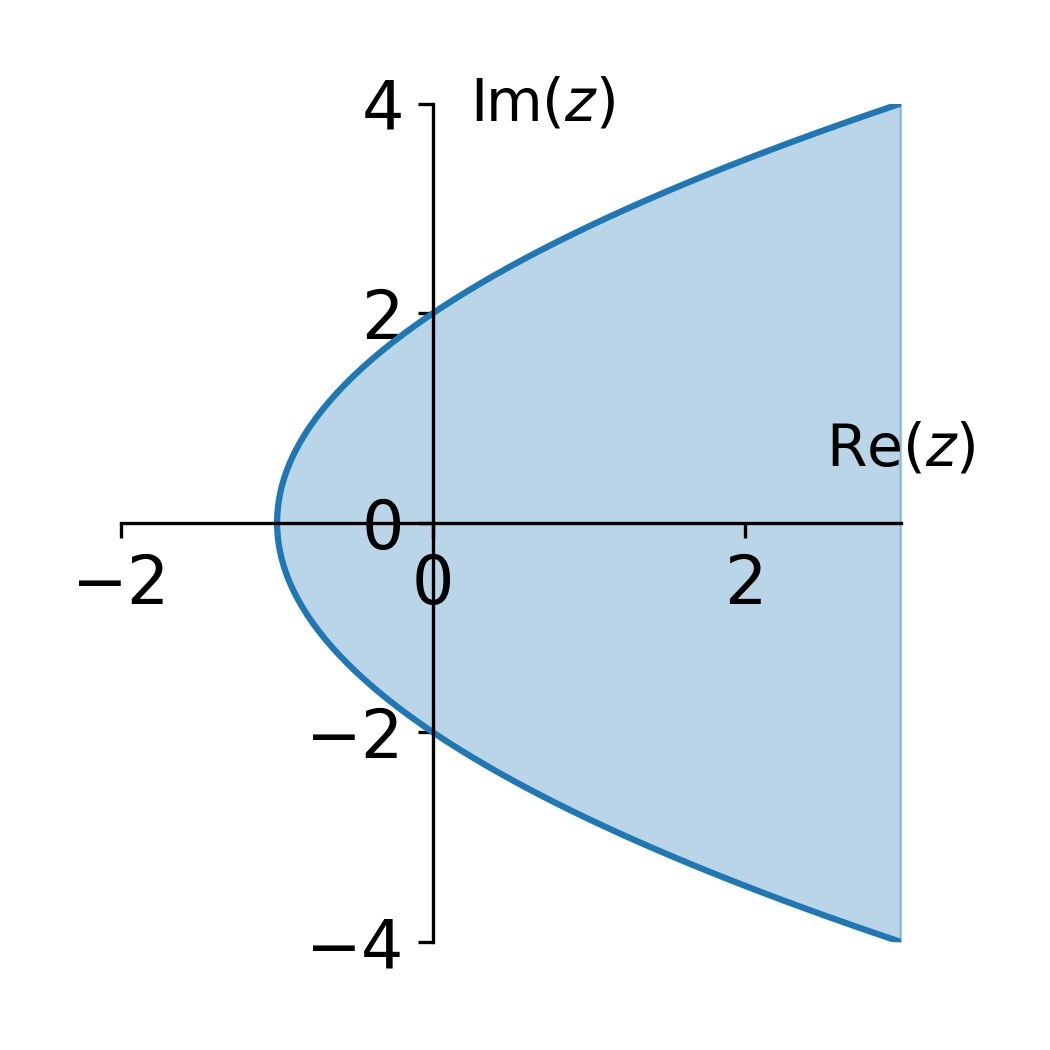
\includegraphics[width=.45\linewidth]{Figures/Section5/loci_ex551b.png}
    \end{center}
\fi

(c) $\left|z-2+i\right|=\blank{\sqrt{{(x-2)}^{2}+{(y+1)}^{2}}}$ so the locus is $\blank{\sqrt{{(x-2)}^{2}+{(y+1)}^{2}}<3}$ or equivalently
\[
\blank{{(x-2)}^{2}+{(y+1)}^{2}<{3}^{2}} \; .
\]
\textit{I.e.} all the points inside a circle with radius $\blank{3}$ and centre $\blank{(2,-1)}$.
\ifcsname insertBlanks\endcsname
    \begin{center}
    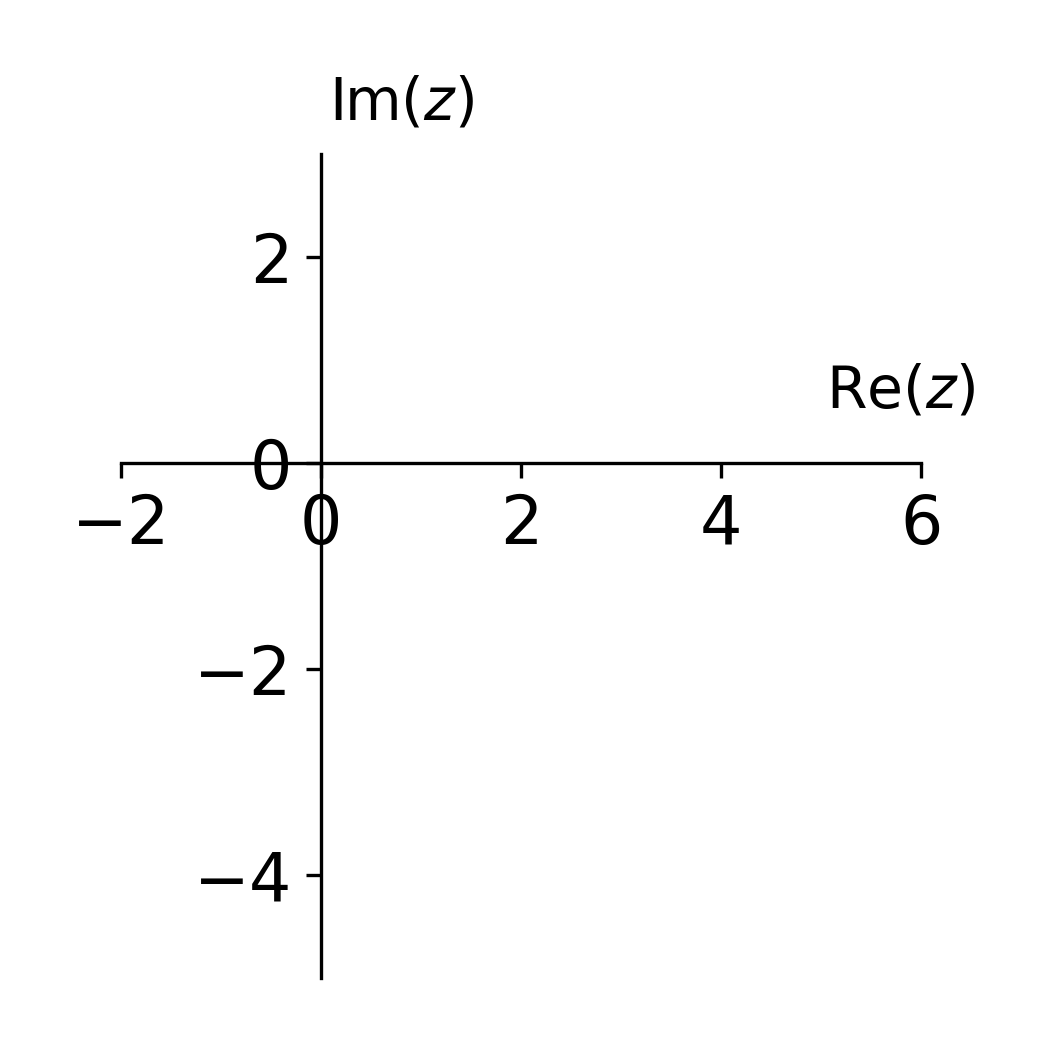
\includegraphics[width=.45\linewidth]{Figures/Section5/loci_ex551c_blank.png}
    \end{center}
\else
    \begin{center}
    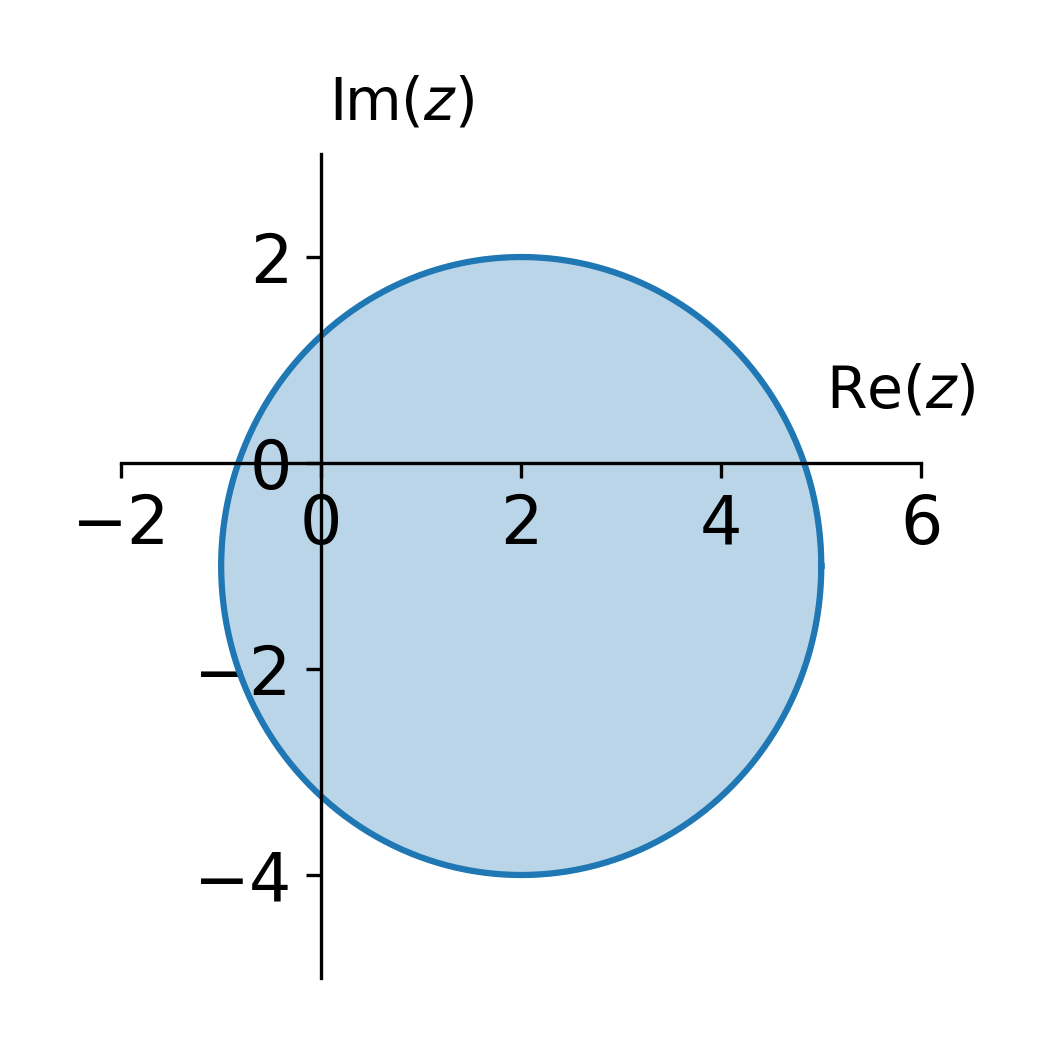
\includegraphics[width=.45\linewidth]{Figures/Section5/loci_ex551c.png}
    \end{center}
\fi
\end{solution}

\begin{exammistake}
    Complex loci may not be intuitive at first and so it is difficult to ``read off'' what the graph will be.  

    \begin{quote}
    \textbf{25/26 Exam Q5(a)(iii)}
    Given $w = 1 + \sqrt{3}i$ \ldots sketch the locus $|z - w| = 1$ on an Argand diagram.
    \end{quote}

    \underline{Answer:} A circle of radius 1 with centre $w$. 

    \vspace{4pt}
    \begin{center}
        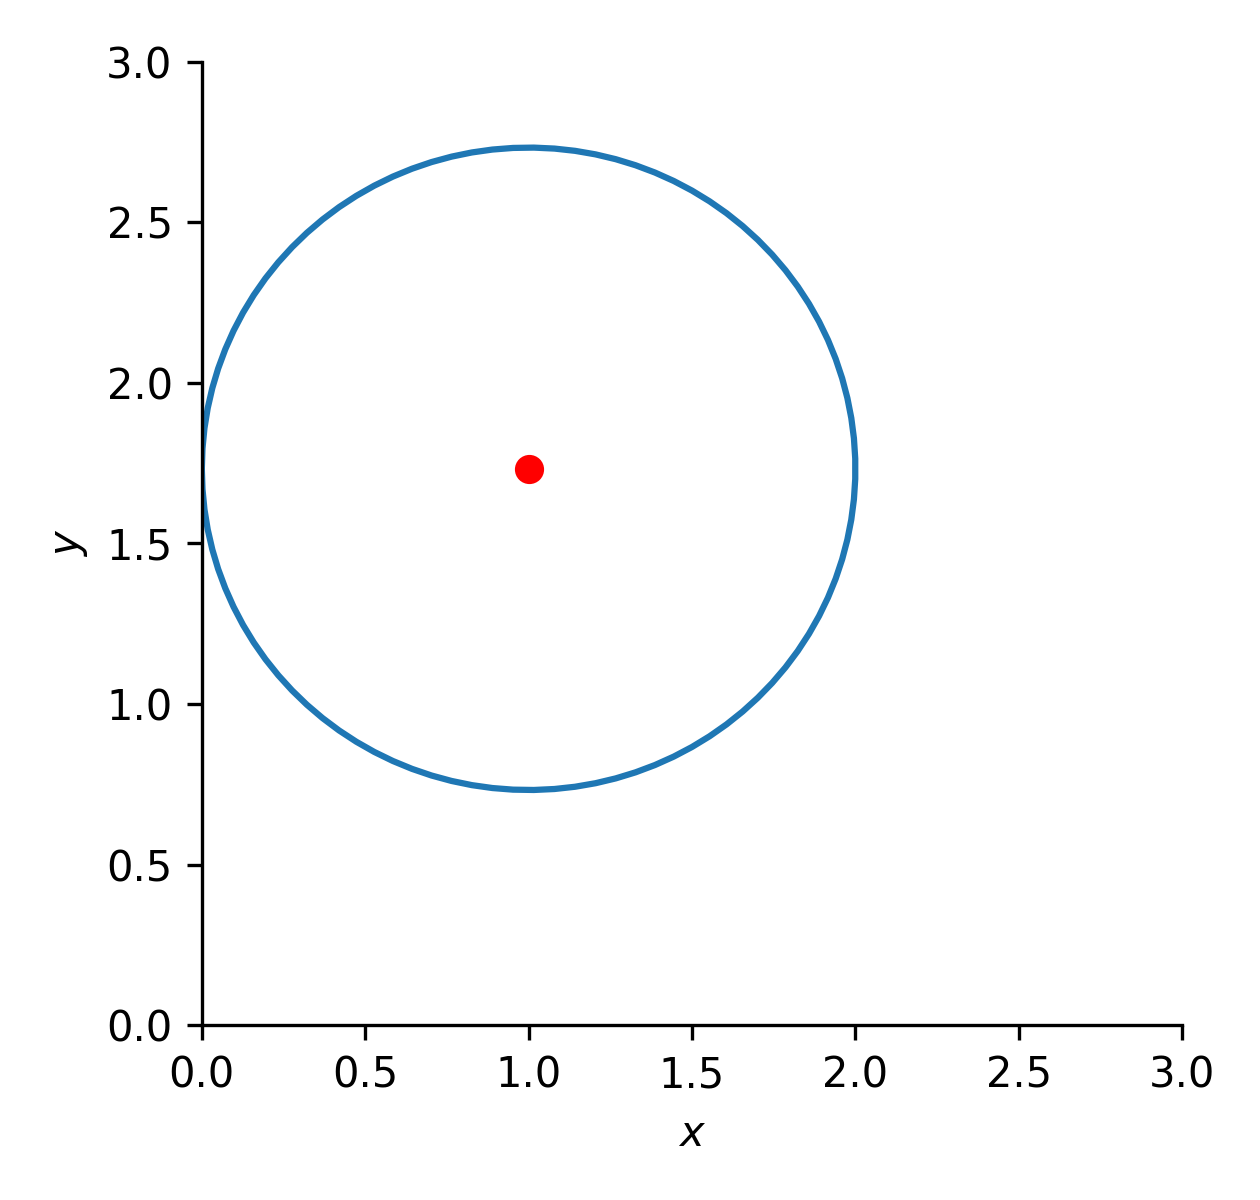
\includegraphics[width=0.4\textwidth]{Figures/Section5/locus_Q5.png}
    \end{center}
    \vspace{4pt}
    
    Many said it was a straight line, several others noticed it was a circle but put the centre at (0,0). \par
    $\rightarrow$ The best approach is to check by substituting in $z=x+yi$ and finding the Cartesian form.
\end{exammistake}

\goodbreak
\begin{recap}{\ref{sec:complex_loci}}
\item Equations and inequalities using complex numbers can be an efficient way to represent sets of points (loci) in $x$-$y$ space.
\item These could be points, lines, or areas depending on the form of the expression, but the resulting expression should not contain $i$.
\item Writing the expression in terms of $x$ and $y$ can help to find the curves
\item Some simple examples are the equation of a circle $\left|z-w\right|=R$ and straight line $\operatorname{Im}\left(z\right)=mRe\left(z+c\right)$ (where $m$ is real)
\end{recap}